\documentclass[twocolumn,a4j]{jsarticle}
\setlength{\topmargin}{-20.4cm}
\setlength{\oddsidemargin}{-10.4mm}
\setlength{\evensidemargin}{-10.4mm}
\setlength{\textwidth}{18cm}
\setlength{\textheight}{26cm}

\usepackage[top=13truemm,bottom=20truemm,left=15truemm,right=15truemm]{geometry}
\usepackage[latin1]{inputenc}
\usepackage{amsmath}
\usepackage{amsfonts}
\usepackage{amssymb}
\usepackage[dvipdfmx]{graphicx}
\usepackage[dvipdfmx]{color}
\usepackage{listings}
\usepackage{listings,jvlisting}
\usepackage{geometry}
\usepackage{framed}
\usepackage{color}
\usepackage[dvipdfmx]{hyperref}
\usepackage{ascmac}
\usepackage{enumerate}
\usepackage{tabularx}
\usepackage{cancel}
\usepackage{scalefnt}

\renewcommand{\figurename}{Fig.}
\renewcommand{\tablename}{Table }

\lstset{
basicstyle={\ttfamily},
identifierstyle={\small},
commentstyle={\smallitshape},
keywordstyle={\small\bfseries},
ndkeywordstyle={\small},
stringstyle={\small\ttfamily},
frame={tb},
breaklines=true,
columns=[l]{fullflexible},
xrightmargin=0zw,
xleftmargin=3zw,
numberstyle={\scriptsize},
stepnumber=1,
numbersep=1zw,
lineskip=-0.5ex
}

\makeatletter
\def\@maketitle
{
\begin{center}
{\LARGE \@title \par}
\end{center}
\begin{flushright}
{\large \@date}\\
{\large{京都工芸繊維大学 工芸科学部 機械工学課程}}\\
{\large \@author}
\end{flushright}
\par\vskip 1.5em
}
\makeatother

\setcounter{tocdepth}{3}

\author{来代 勝胤 / Masatsugu KITADAI}
\title{令和3年度 1月度 報告書}
\date{2022/1/25}

\begin{document}
\columnseprule=0.1mm

\maketitle
\section*{報告内容}
\begin{enumerate}[1.]
    \item 進捗状況
    \item 実験装置の製作
    \item 実験の実施と結果
    \item 補正理論と適用結果
    \item 今月の進捗と今後の予定
\end{enumerate}

\section{進捗状況}
今月は,12月に行った模擬実験方法を基準に自動ステージを用いて
製作した実験装置を使用して性能評価実験を行った.
また,実験結果に対しての補正理論を作成し,それを用いてデータ処理を行った.

\section{実験装置の製作}

前回の模擬実験では,人為的操作を含む実験を行ったが,
再現性が保証できないことや実験を複数回行うことが困難であることから
自動一軸ステージ,自動回転ステージを用いて実験を自動化し,
\textgt{可能な限りの人為的操作を削除すること,実験回数の確保すること}
を目標に新たに実験装置を製作した.
以下のFig.に実験装置の3Dモデル,Fig.に製作した実験装置の写真を示す.

\begin{figure}[htbp]
    \footnotesize
    \begin{center}
        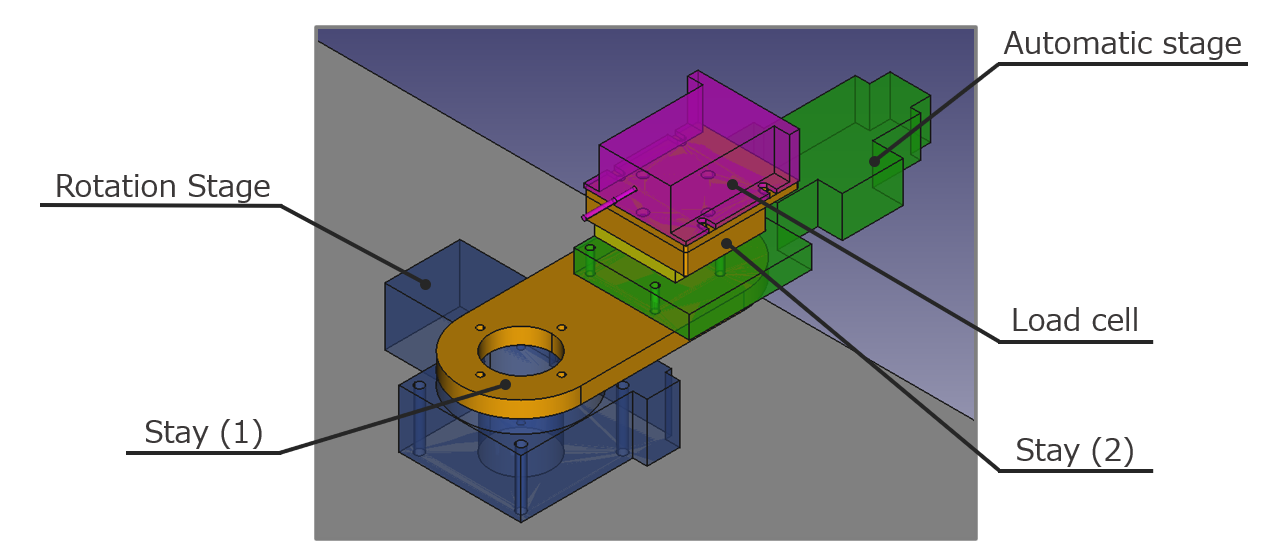
\includegraphics[width=85mm]{../images/21-1.png}
        \caption{Automatic experimental device (3D CAD)}
        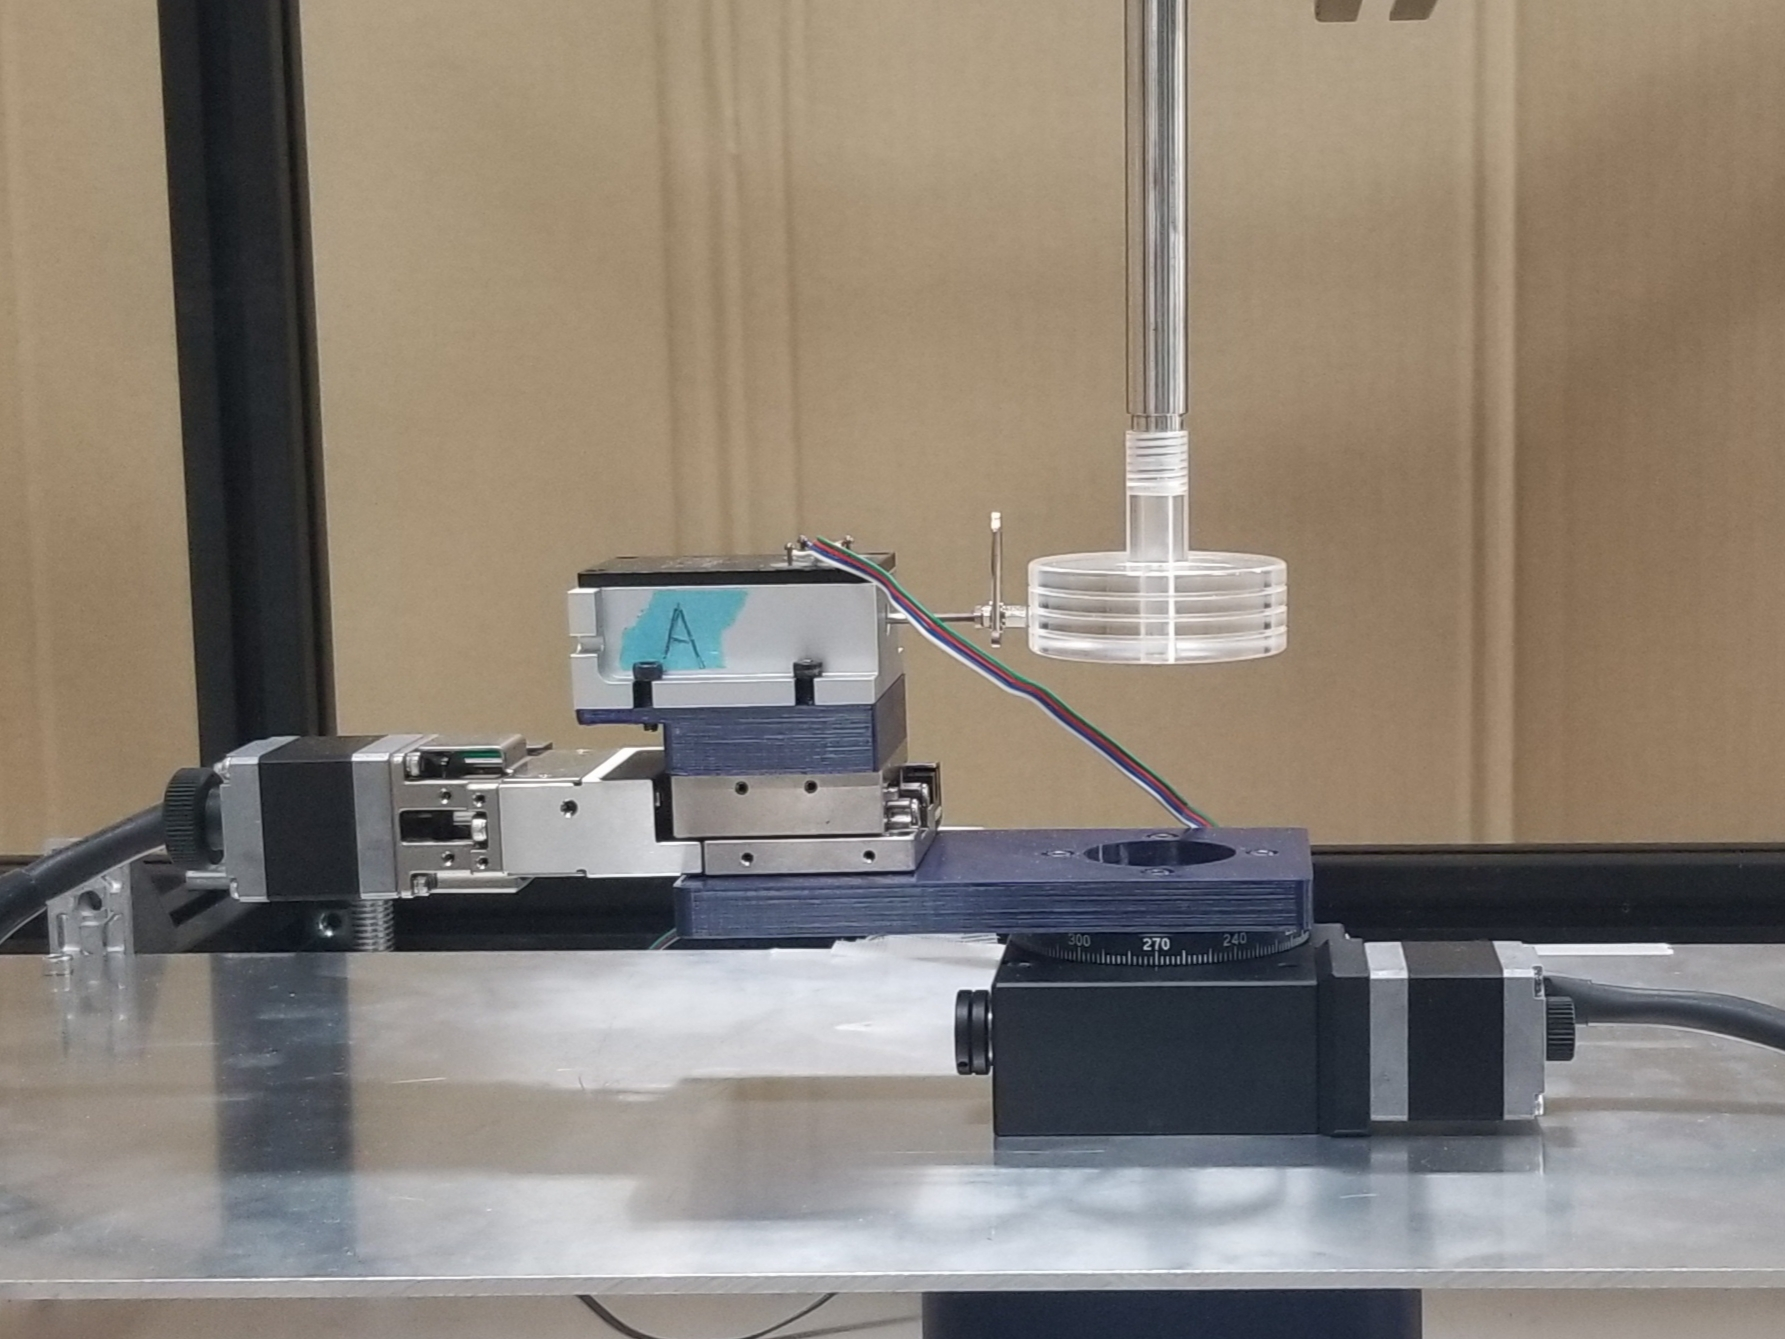
\includegraphics[width=55mm]{../images/device_01.jpg}
        \caption{Automatic experimental device (Photo)}
    \end{center}
\end{figure}

\newpage

\section{実験の実施と結果}

\subsection{実験条件}

今回の実験は以下の条件で行った.
また,実験の測定準備・測定手順においては前回の模擬実験と同様である.

\begin{table}[htbp]
    \begin{center}
        \begin{tabular}{|p{30mm}|p{20mm}|p{30}|}
            \hline
            \multicolumn{1}{|c|}{\textgt{項目}} & \multicolumn{1}{|c|}{\textgt{条件数}} & \multicolumn{1}{|c|}{\textgt{備考}}           \\ \hline
            \multicolumn{1}{|c|}{測定角度}      & \multicolumn{1}{|c|}{24}              & \multicolumn{1}{|c|}{\textgt{15度ごとの測定}} \\ \hline
            \multicolumn{1}{|c|}{試行回数}      & \multicolumn{1}{|c|}{5}               & \multicolumn{1}{|c|}{\textgt{}}               \\ \hline
        \end{tabular}
    \end{center}
\end{table}

\subsection{実験結果}
今回の実験結果について以下のFig.~Fig.に示す.
なお,ここでは実験1回目における 0 [deg],45 [deg]についての結果を示している.

\begin{figure}[htbp]
    \footnotesize
    \begin{center}
        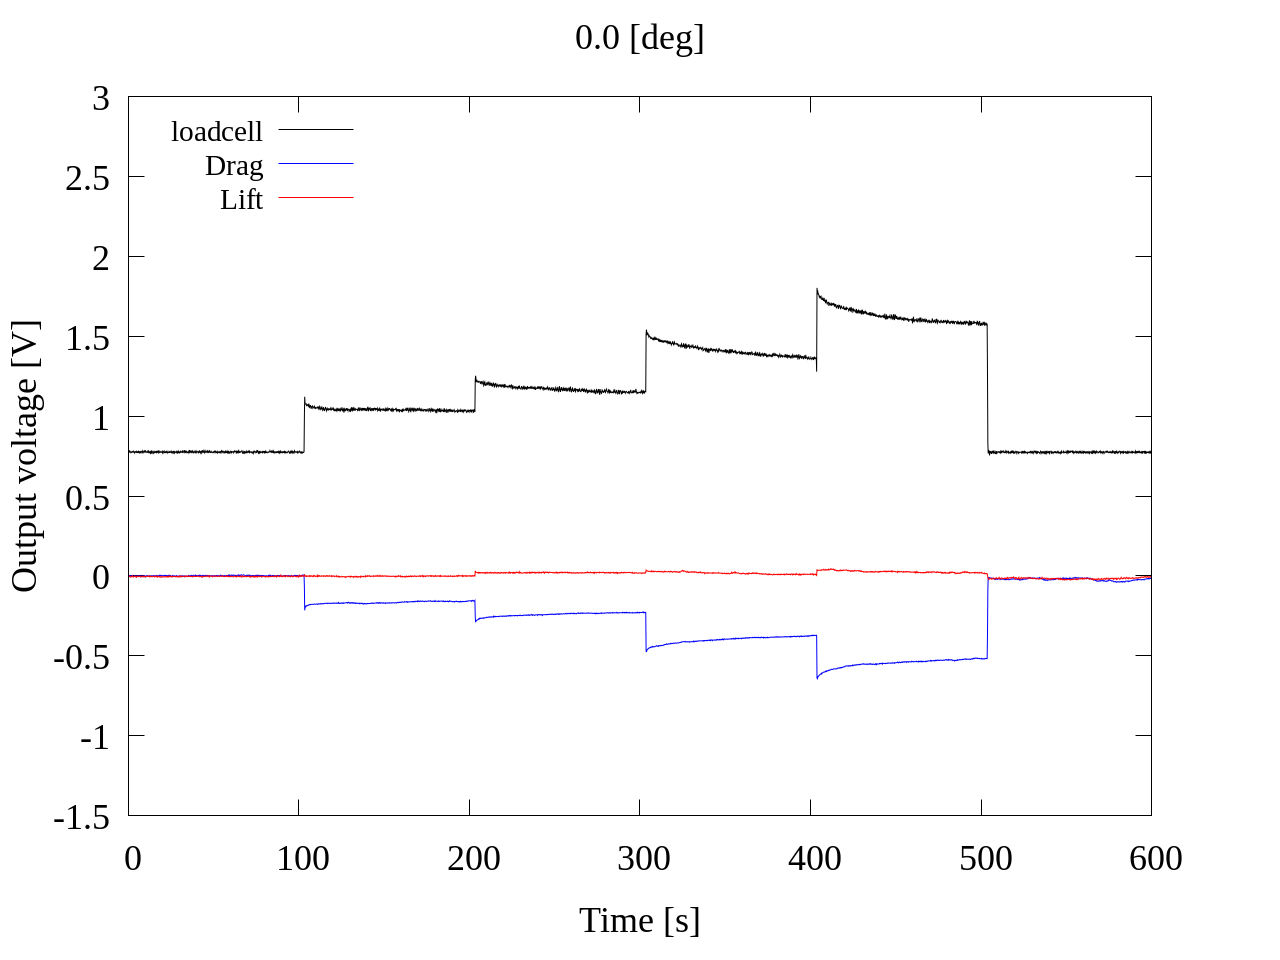
\includegraphics[width=82mm]{../../../02_workspace/result/2-1/plot/01-3_allsensors/01_allsensors_0.png}
        \caption{Output voltage (0 [deg])}
        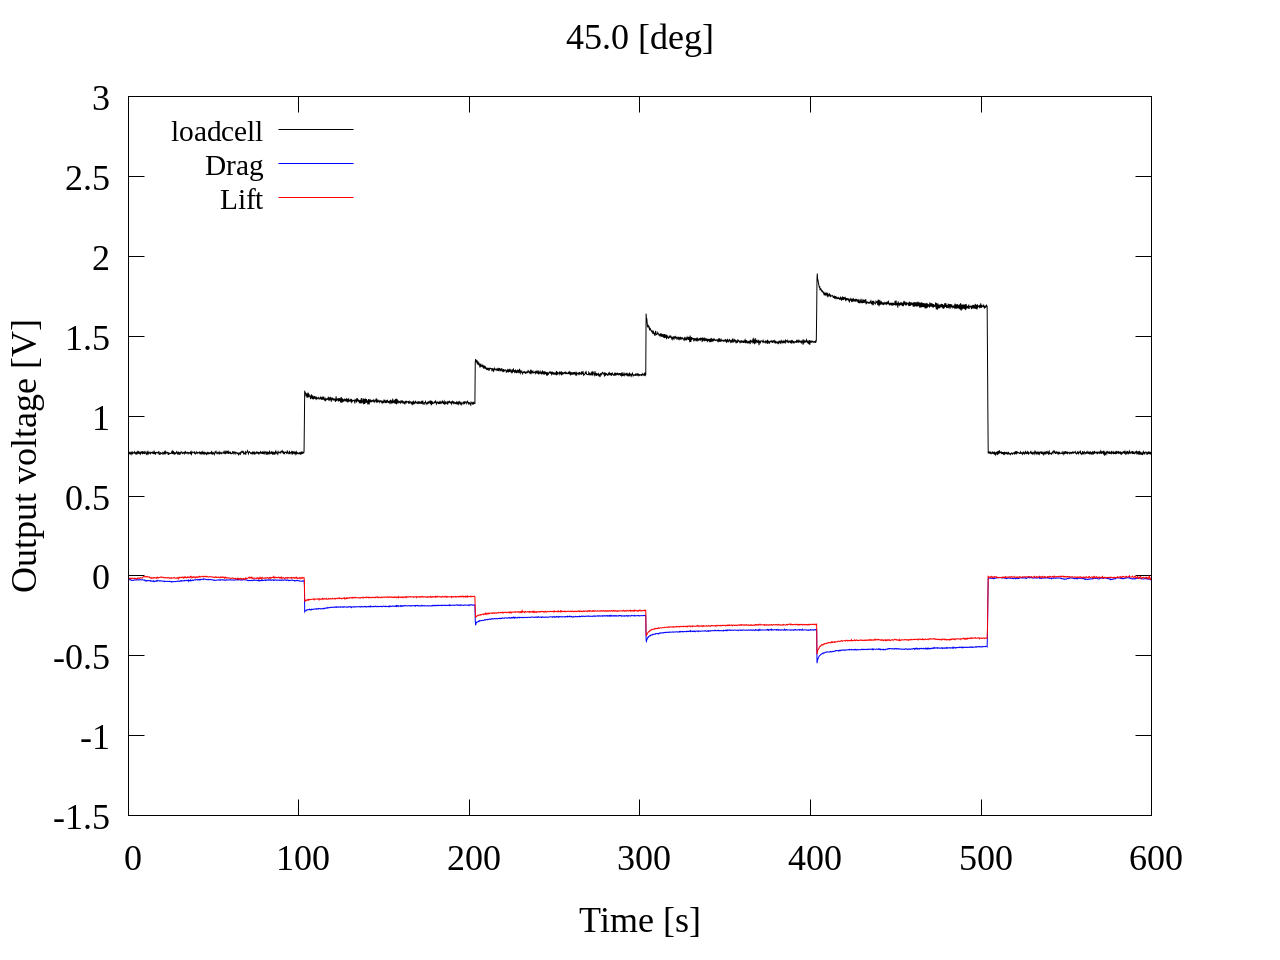
\includegraphics[width=82mm]{../../../02_workspace/result/2-1/plot/01-3_allsensors/01_allsensors_450.png}
        \caption{Output voltage (45 [deg])}
    \end{center}
\end{figure}

\newpage
Fig.4,Fig.5より,自動ステージを用いることによってノイズが除去されていることがわかる.
また,自動一軸ステージが移動した直後から出力電圧の減衰が見られる場合があるが,
同様の変化がロードセルおよびひずみセンサにみられることから大きな問題ではないと考える.\\

\subsection{出力電圧勾配による評価}

実験結果の処理手順に沿って出力電圧勾配を算出する.
1~5回目の実験結果について,以下のFig.5~Fig.9に示す.

\begin{figure}[htbp]
    \footnotesize
    \begin{center}
        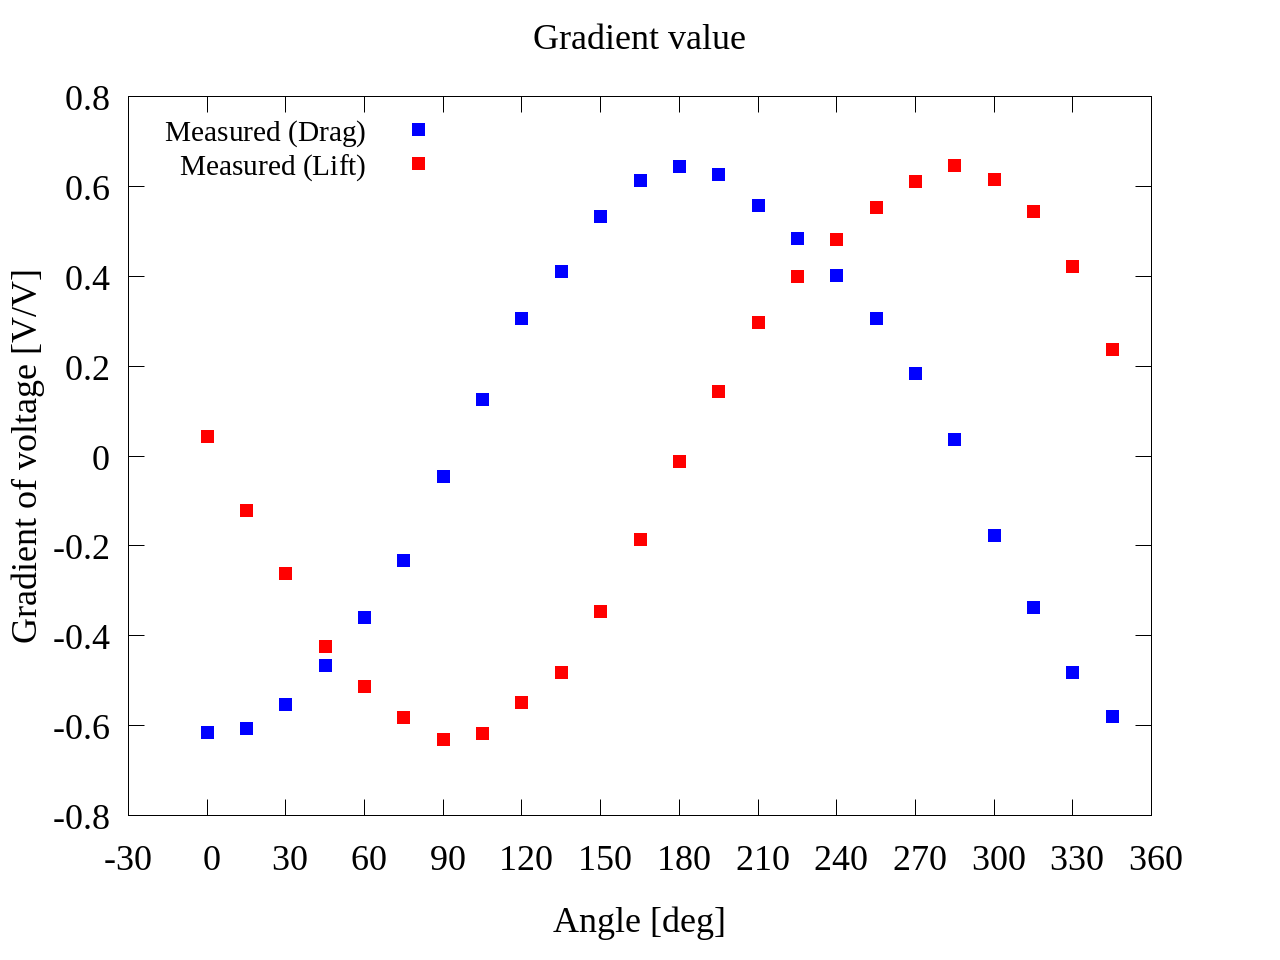
\includegraphics[width=80mm]{../../../02_workspace/result/2-1/plot/05/05_summary-wave.png}
        \caption{Gradient of output voltage (1st)}
        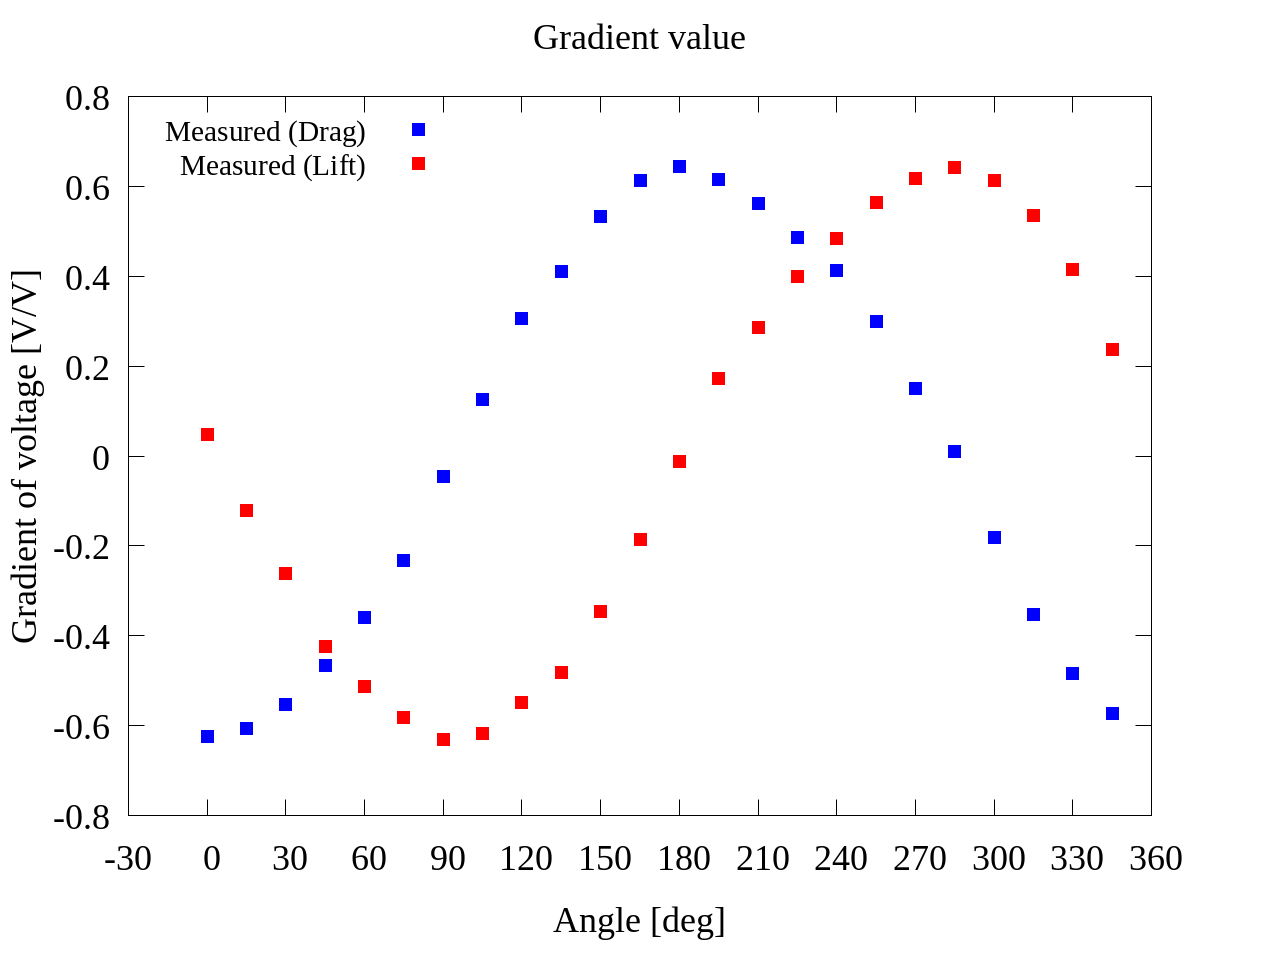
\includegraphics[width=80mm]{../../../02_workspace/result/2-2/plot/05/05_summary-wave.png}
        \caption{Gradient of output voltage (2nd)}
        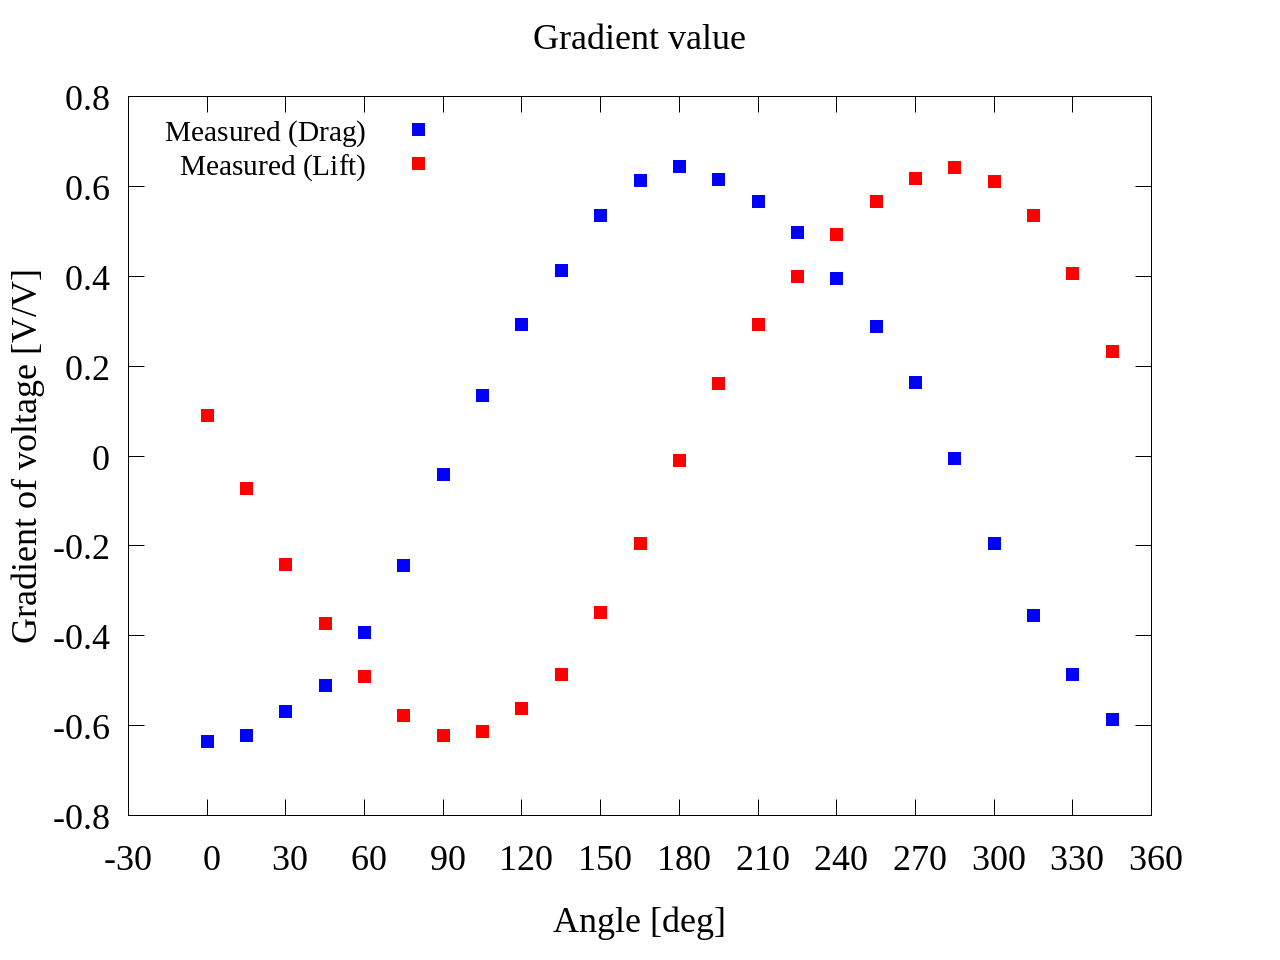
\includegraphics[width=80mm]{../../../02_workspace/result/2-3/plot/05/05_summary-wave.png}
        \caption{Gradient of output voltage (3rd)}
    \end{center}
\end{figure}

\begin{figure}[htbp]
    \footnotesize
    \begin{center}
        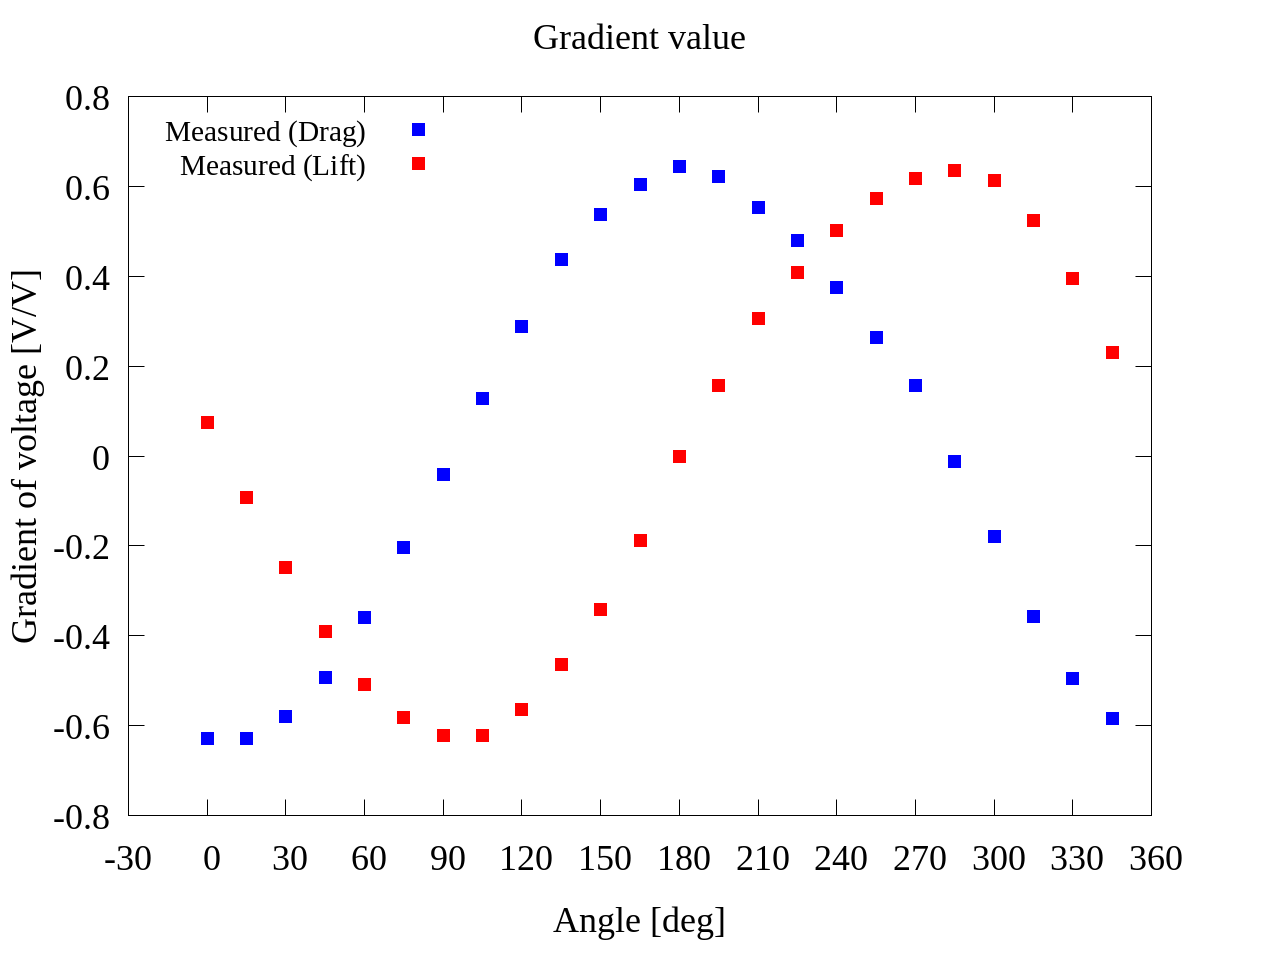
\includegraphics[width=80mm]{../../../02_workspace/result/2-4/plot/05/05_summary-wave.png}
        \caption{Gradient of output voltage (4th)}
        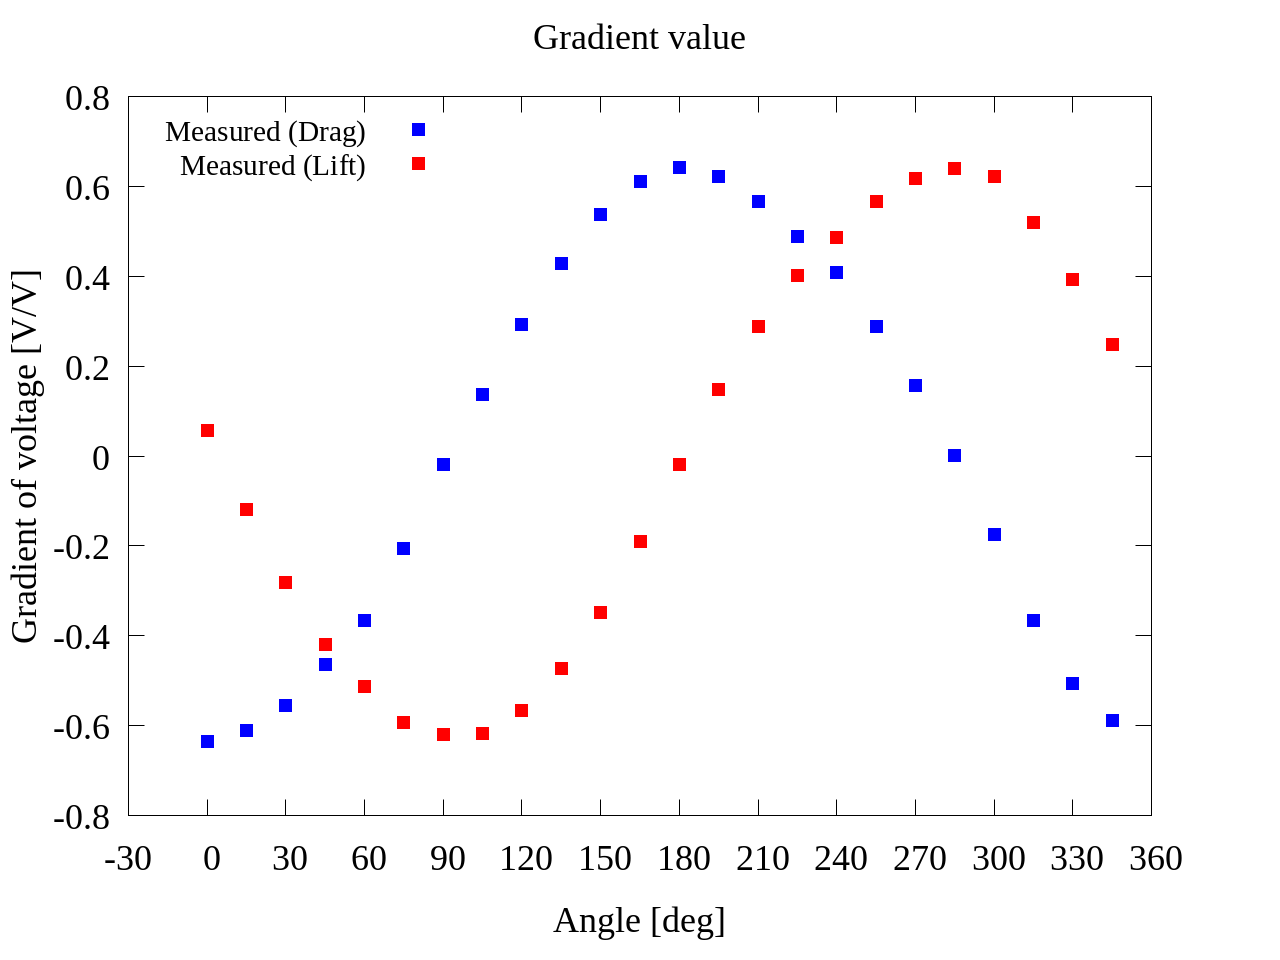
\includegraphics[width=80mm]{../../../02_workspace/result/2-5/plot/05/05_summary-wave.png}
        \caption{Gradient of output voltage (5th)}
    \end{center}
\end{figure}

出力電圧勾配に対する補正処理ついては実験結果の一般性を保証するため
計5回の実験結果の平均値を用いることとする.
その平均値を示した図をFig.10に示す.

\begin{figure}[htbp]
    \footnotesize
    \begin{center}
        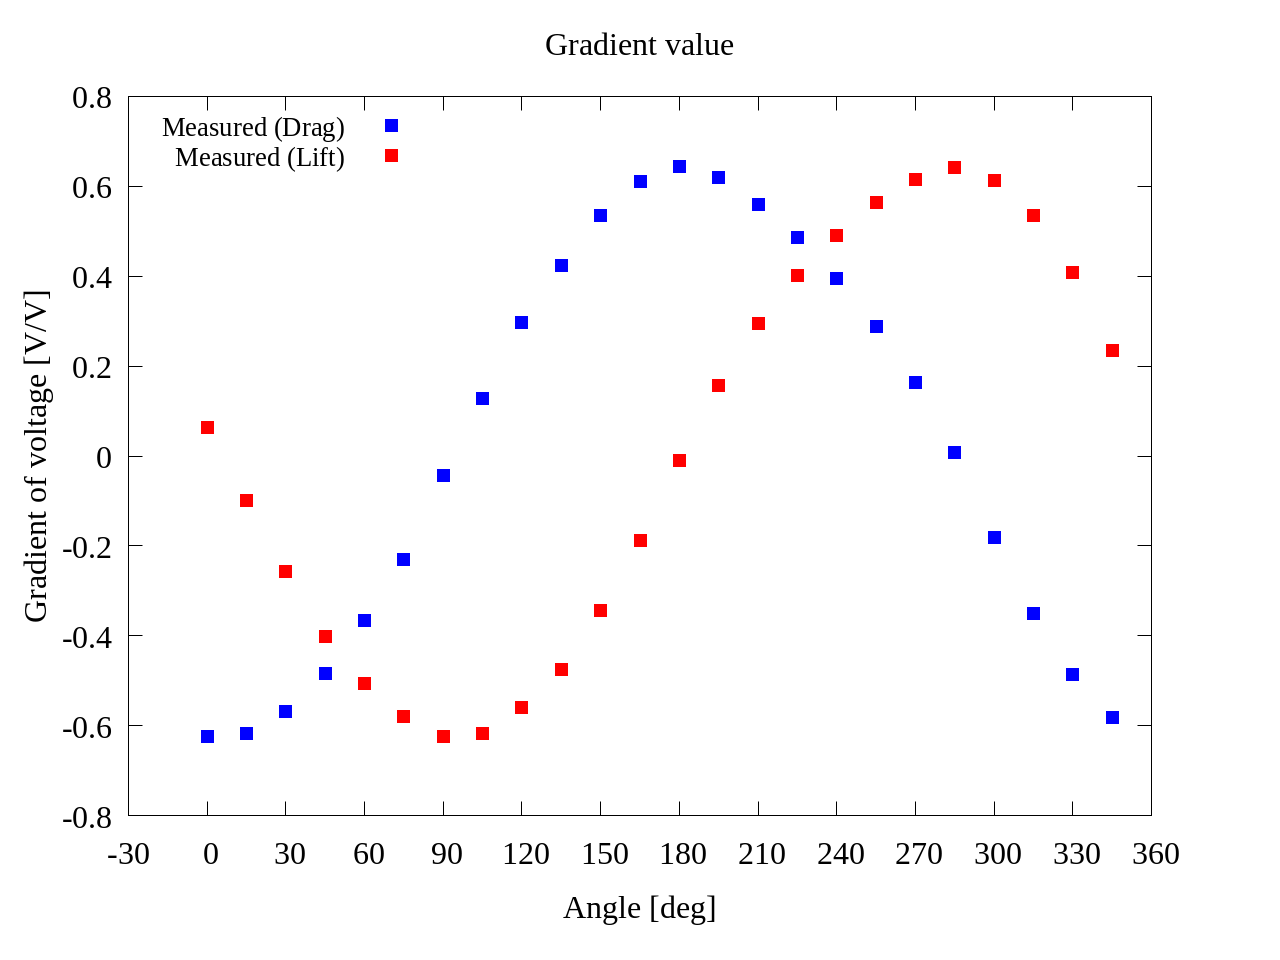
\includegraphics[width=80mm]{../../../02_workspace/result/2-ex/plot/05/05_summary-wave.png}
        \caption{Gradient of output voltage (Average)}
    \end{center}
\end{figure}

また,それそれの角度の値について
抗力方向の出力電圧勾配を$v_d$,揚力方向を$v_l$として次ページのTable 1に示す.

\begin{table}[htbp]
    \begin{center}
        \caption{Result summary}
        \begin{tabular}{|p{20mm}|p{20mm}|p{20mm}|}
            \hline
            \multicolumn{1}{|c|}{\textgt{Angle [deg]}} & \multicolumn{1}{|c|}{\textgt{$v_d$ [V/V]}} & \multicolumn{1}{|c|}{\textgt{$v_l$ [V/V]}} \\ \hline
            \multicolumn{1}{|c|}{0}                    & \multicolumn{1}{|r|}{-0.627}               & \multicolumn{1}{|r|}{ 0.063}               \\ \hline
            \multicolumn{1}{|c|}{15}                   & \multicolumn{1}{|r|}{-0.617}               & \multicolumn{1}{|r|}{-0.103}               \\ \hline
            \multicolumn{1}{|c|}{30}                   & \multicolumn{1}{|r|}{-0.566}               & \multicolumn{1}{|r|}{-0.261}               \\ \hline
            \multicolumn{1}{|c|}{45}                   & \multicolumn{1}{|r|}{-0.479}               & \multicolumn{1}{|r|}{-0.405}               \\ \hline
            \multicolumn{1}{|c|}{60}                   & \multicolumn{1}{|r|}{-0.365}               & \multicolumn{1}{|r|}{-0.508}               \\ \hline
            \multicolumn{1}{|c|}{75}                   & \multicolumn{1}{|r|}{-0.226}               & \multicolumn{1}{|r|}{-0.582}               \\ \hline
            \multicolumn{1}{|c|}{90}                   & \multicolumn{1}{|r|}{-0.038}               & \multicolumn{1}{|r|}{-0.624}               \\ \hline
            \multicolumn{1}{|c|}{105}                  & \multicolumn{1}{|r|}{0.131}                & \multicolumn{1}{|r|}{-0.618}               \\ \hline
            \multicolumn{1}{|c|}{120}                  & \multicolumn{1}{|r|}{0.296}                & \multicolumn{1}{|r|}{-0.560}               \\ \hline
            \multicolumn{1}{|c|}{135}                  & \multicolumn{1}{|r|}{0.425}                & \multicolumn{1}{|r|}{-0.474}               \\ \hline
            \multicolumn{1}{|c|}{150}                  & \multicolumn{1}{|r|}{0.536}                & \multicolumn{1}{|r|}{-0.345}               \\ \hline
            \multicolumn{1}{|c|}{165}                  & \multicolumn{1}{|r|}{0.611}                & \multicolumn{1}{|r|}{-0.189}               \\ \hline
            \multicolumn{1}{|c|}{180}                  & \multicolumn{1}{|r|}{0.643}                & \multicolumn{1}{|r|}{-0.011}               \\ \hline
            \multicolumn{1}{|c|}{195}                  & \multicolumn{1}{|r|}{0.620}                & \multicolumn{1}{|r|}{0.156}                \\ \hline
            \multicolumn{1}{|c|}{210}                  & \multicolumn{1}{|r|}{0.561}                & \multicolumn{1}{|r|}{0.294}                \\ \hline
            \multicolumn{1}{|c|}{225}                  & \multicolumn{1}{|r|}{0.487}                & \multicolumn{1}{|r|}{0.402}                \\ \hline
            \multicolumn{1}{|c|}{240}                  & \multicolumn{1}{|r|}{0.399}                & \multicolumn{1}{|r|}{0.489}                \\ \hline
            \multicolumn{1}{|c|}{255}                  & \multicolumn{1}{|r|}{0.289}                & \multicolumn{1}{|r|}{0.565}                \\ \hline
            \multicolumn{1}{|c|}{270}                  & \multicolumn{1}{|r|}{0.163}                & \multicolumn{1}{|r|}{0.616}                \\ \hline
            \multicolumn{1}{|c|}{285}                  & \multicolumn{1}{|r|}{0.006}                & \multicolumn{1}{|r|}{0.641}                \\ \hline
            \multicolumn{1}{|c|}{300}                  & \multicolumn{1}{|r|}{-0.181}               & \multicolumn{1}{|r|}{0.615}                \\ \hline
            \multicolumn{1}{|c|}{315}                  & \multicolumn{1}{|r|}{-0.353}               & \multicolumn{1}{|r|}{0.532}                \\ \hline
            \multicolumn{1}{|c|}{330}                  & \multicolumn{1}{|r|}{-0.490}               & \multicolumn{1}{|r|}{0.406}                \\ \hline
            \multicolumn{1}{|c|}{345}                  & \multicolumn{1}{|r|}{-0.582}               & \multicolumn{1}{|r|}{0.237}                \\ \hline
        \end{tabular}
    \end{center}
\end{table}

\newpage

\section{補正理論と適用結果}

作用力測定装置から得た抗力方向および揚力方向における出力電圧$V_D$,$V_L$を
正規座標系の$x$軸方向および$y$軸方向の荷重$F_x$,$F_y$に換算する際に,
出力電圧$V_D$,$V_L$と$F_x$,$F_y$の関係性を明らかにするための校正実験を
行う必要がある.\\

\subsection{作用力測定装置と校正実験装置の関係}
作用力測定装置と校正実験装置の設置位置によって校正実験結果は大きく変動するため,
その影響を考慮し,補正処理を行う必要がある.
このとき以下のような要因が,校正実験結果への影響を与えていると考えられる.

\begin{enumerate}[(1)]
    \item 作用力測定装置のひずみセンサの取付
    \item 作用力測定装置の回流水槽への設置
    \item 作用力測定装置と校正装置の設置
\end{enumerate}

\newpage

ここで,水流に対する座標系を正規座標系 $(x,y)$,
作用力測定装置の座標系を座標系(1) $(x',y')$,
校正装置の座標系を座標系(2) $(x,'' y'')$とする.

このとき,(1) 作用力測定装置のひずみセンサの取付,
(2) 作用力測定装置の回流水槽への取付 の際に正確に取り付けられていることを保証できないことから
座標系[1]は正規座標系に対して
$x'$軸は$x$軸から$\theta_x$,$y'$軸は$y$軸から$\theta_y$だけ回転している.
また,座標系[2]は正規座標系に対して
$x''$軸は$x$軸から$y$方向に$\Delta x$,
$y''$軸は$y$軸から$x$方向に$\Delta y$だけオフセットを持つ状態となると考えられる.

\begin{figure}[htbp]
    \footnotesize
    \begin{center}
        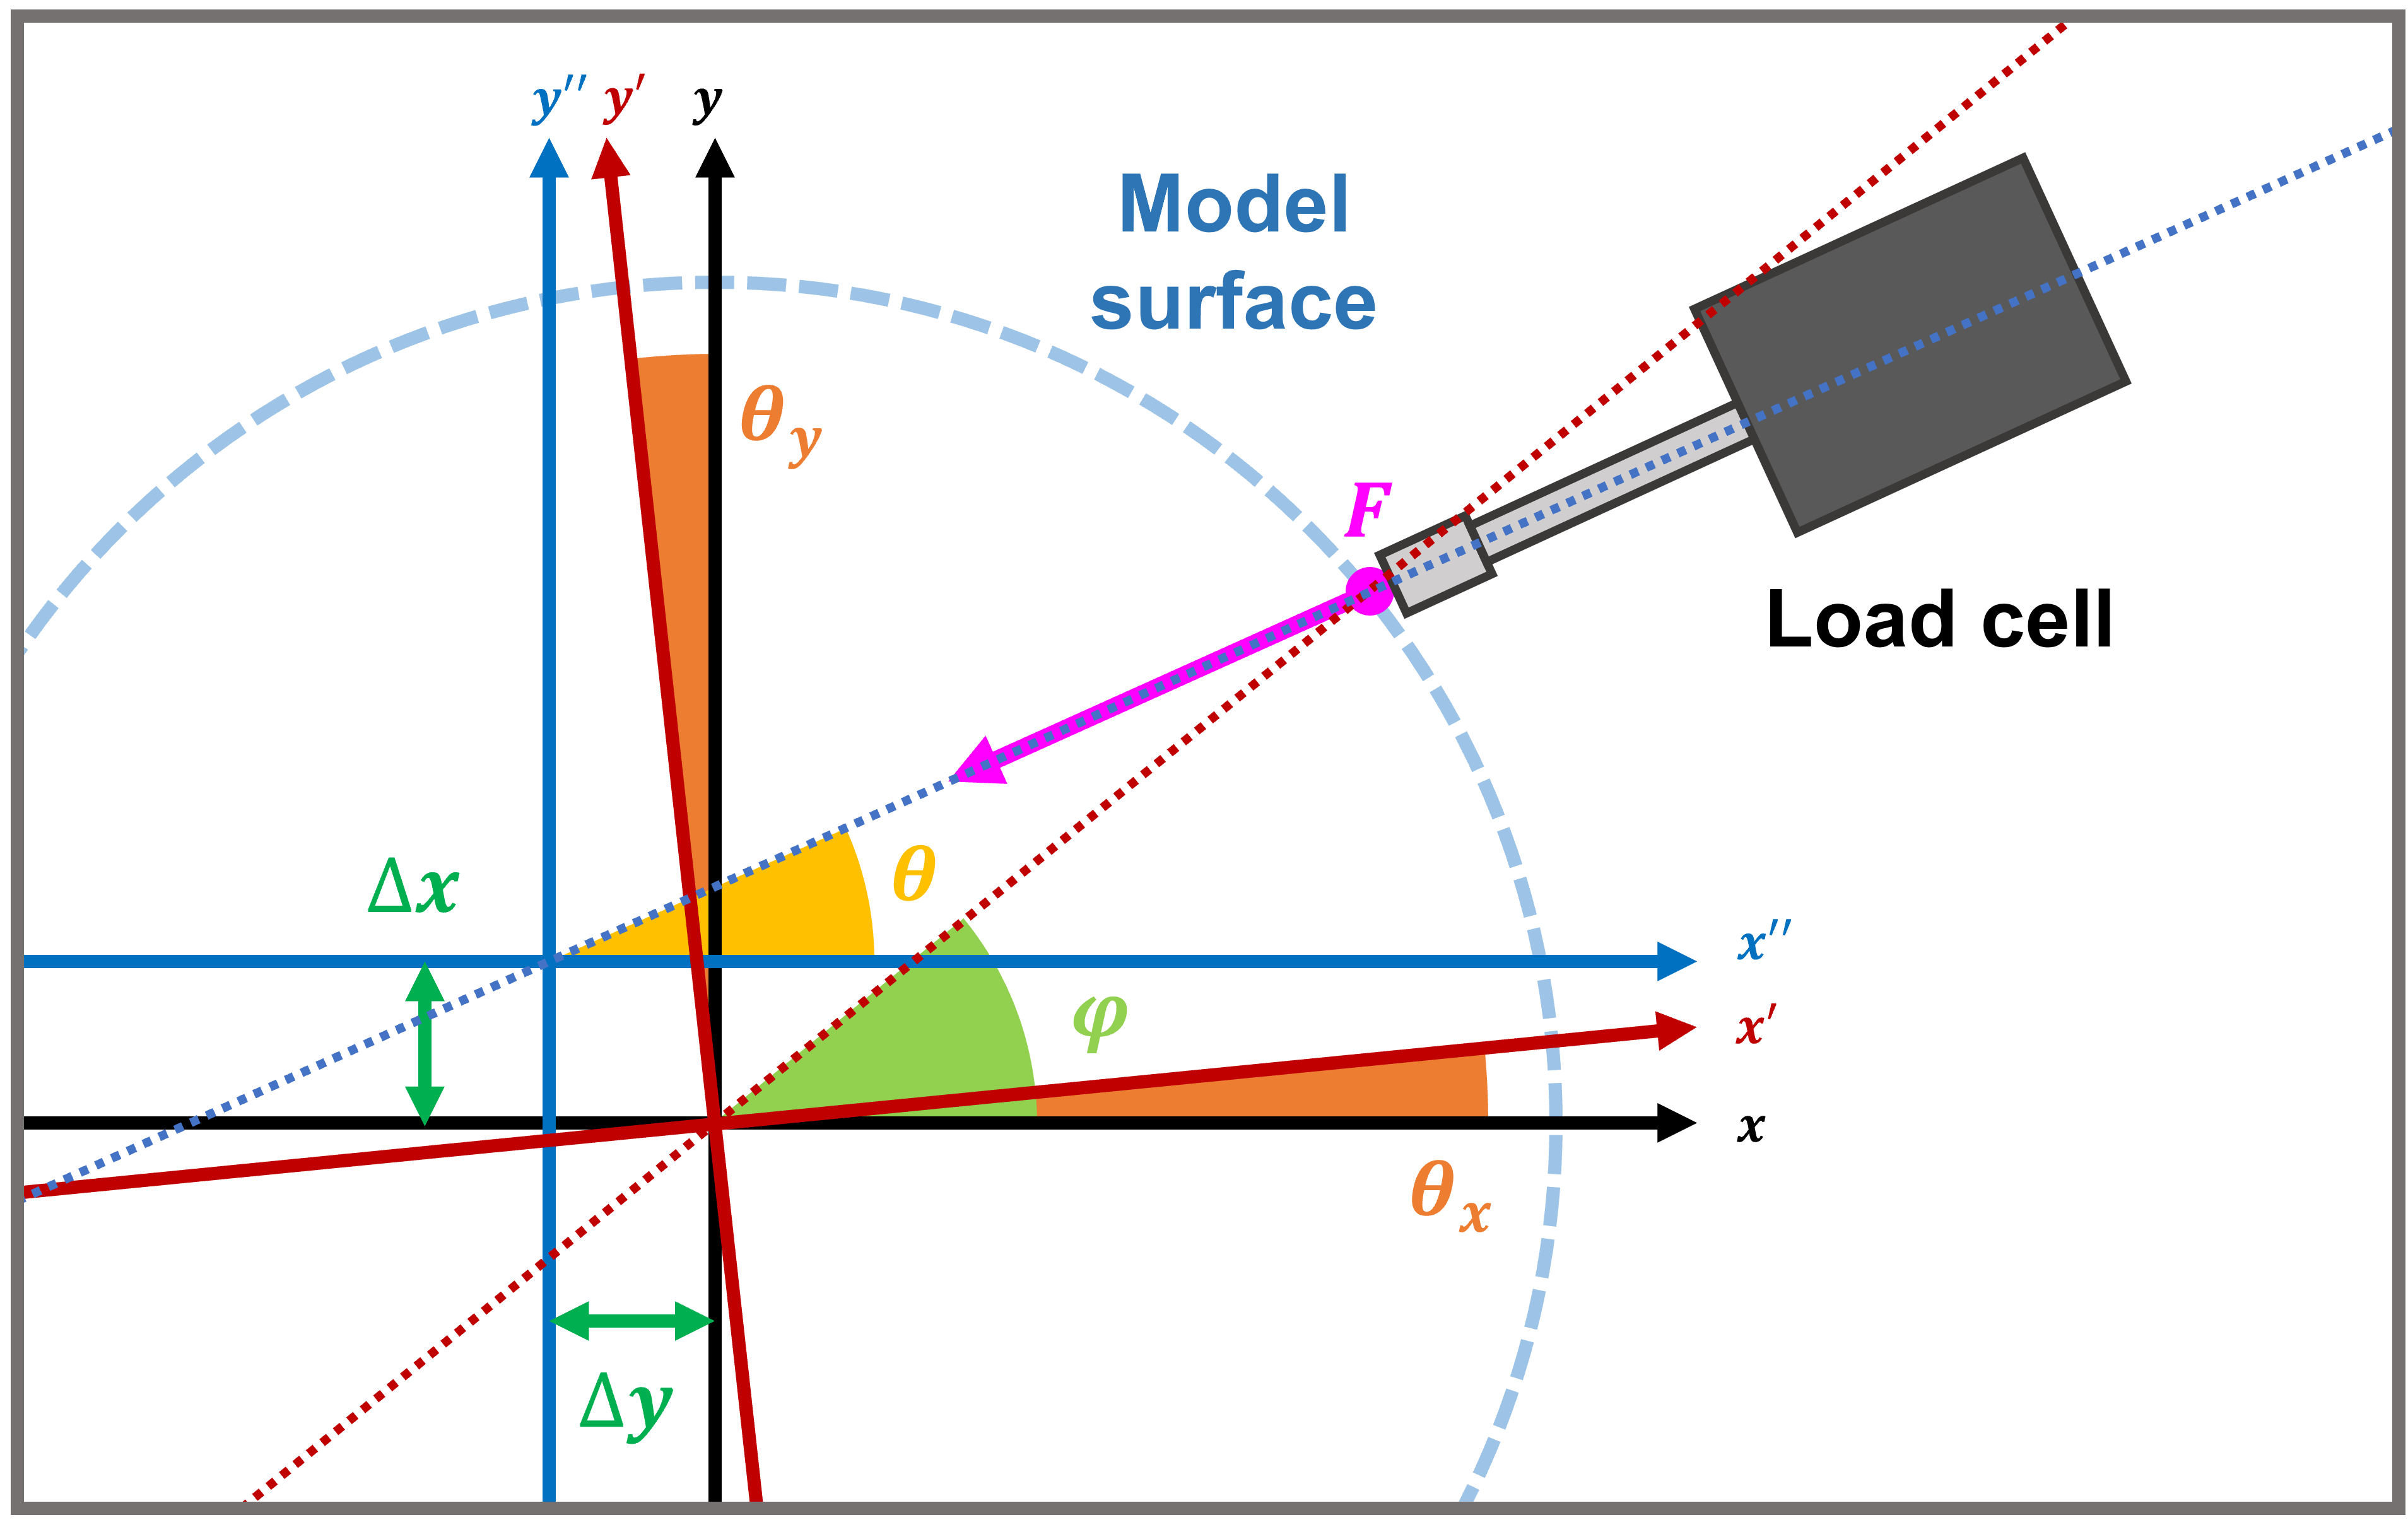
\includegraphics[width=80mm]{../images/31-1.png}
        \caption{}
    \end{center}
\end{figure}

\subsection{座標系の回転における補正理論}
\vskip \baselineskip

\subsubsection{回転角$\theta_x$,$\theta_y$の算出}

はじめに,回転角$\theta_{x}$,$\theta_{y}$を算出する.
理論式における$v_{x\;\mathrm{theory}}$及び$v_{y\;\mathrm{theory}}$は正弦波とその位相差で表すことができる.
したがって,校正実験結果の各角度の出力電圧勾配においても同様の正弦波と
その位相差で表すことが可能であると予想することができる.
このとき,離散フーリエ変換を適用し,
波数1の成分について,実部を$Re$,虚部を$Im$として
位相角$\phi$を求めることができる.

\begin{align*}
    \phi = \arctan \left(\frac{Im}{Re}\right) \cdot \frac{180}{\pi}
\end{align*}
\vskip \baselineskip

抗力方向の結果から得られた位相角を$\phi_1$,揚力方向から得られた位相角を$\phi_2$と
するとき,抗力方向の出力電圧勾配$v_d$と
正規座標系における$x$軸方向の出力電圧勾配の理論値$v_{x\;\mathrm{theory}}$との位相差
$\theta_x$,
揚力方向の出力電圧勾配$v_l$と
正規座標系における$y$軸方向の出力電圧勾配の理論値$v_{y\;\mathrm{theory}}$との位相差
$\theta_y$を以下のように表される.

\begin{align*}
    \theta_x = \pi - \phi_1 \\
    \theta_y = \frac{\pi}{2} - \phi_2
\end{align*}
\vskip \baselineskip

したがって,$x'$軸,$y'$軸は左回りを正方向として,それぞれ$\theta_x$,$\theta_y$だけ
回転していることとなる.
また,作用力測定装置に取り付けられた抗力・揚力方向のひずみセンサの取付角$\phi_s$は
位相角$\phi_1$,$\phi_2$より求めることができる.

\begin{align*}
    \phi_s = \left| \phi_1 - \phi_2 \right|
\end{align*}

\subsubsection{出力電圧勾配の座標変換}

位相角$\theta_x$,$\theta_y$が求められたことから,
それらを用いて出力電圧勾配の座標変換を行う.
ここで,座標系[1]の$x'$軸,$y'$軸を
それぞれ$f_{x}\left(x\right)$,$f_{y}\left(x\right)$として,
正規座標軸の$x$を用いた式で表す.

\begin{figure}[htbp]
    \footnotesize
    \begin{center}
        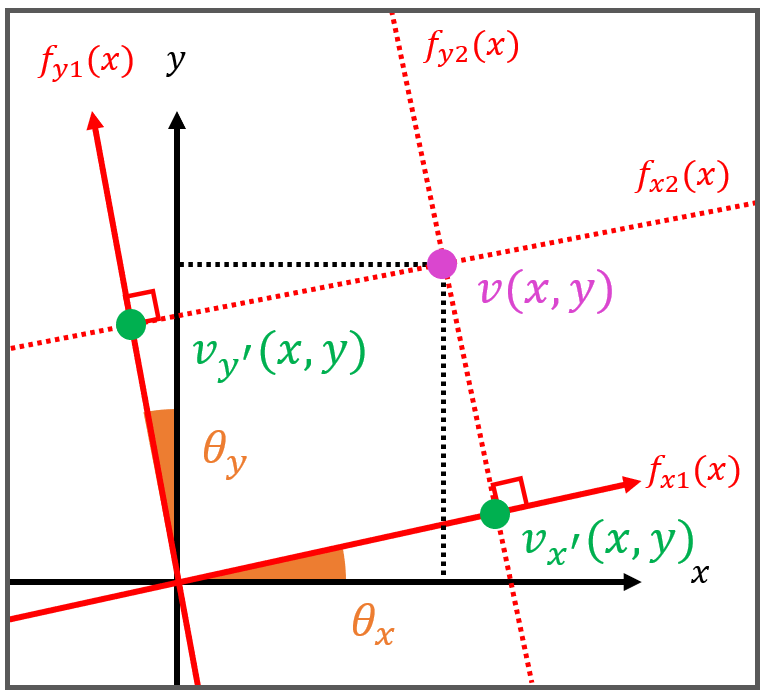
\includegraphics[width=75mm]{../images/33-2.png}
        \caption{}
    \end{center}
\end{figure}

算出した位相角$\theta_x$,$\theta_y$より,$f_{x}\left(x\right)$,$f_{y}\left(x\right)$は
以下のように表される.

\begin{align*}
    f_{x}\left(x\right) & = \tan \theta_x \; x            \\
    f_{y}\left(x\right) & = - \frac{1}{\tan \theta_y}\; x
\end{align*}
\vskip \baselineskip

このとき,作用力$F$は,Fig.に示す点$F$の座標を表すベクトルと考えることができる.
また,その座標はFig.より,$f_{x}\left(x\right)$,$f_{y}\left(x\right)$の法線で,
点$v_{x'}$,$v_{y'}$を通る直線,
$f_{x2}\left(x\right)$,$f_{y2}\left(x\right)$の交点であることがわかる.\par
ここで,ひずみゲージから得ることのできる出力電圧の傾きから,
$v_{x'}$,$v_{y'}$のベクトルの大きさ$|\boldsymbol{v_{x'}}|$,$|\boldsymbol{v_{y'}}|$を
得ることができる.
角度$\theta_x$,$\theta_y$が求められていることから,
点$v_{x'}$,$v_{y'}$の座標を以下のように求めることができる.

\begin{align*}
    v_{x'} \left(x ,y\right) & = \left(|\boldsymbol{v_{x'}}| \cos \theta_x,\; |\boldsymbol{v_{x'}}| \sin \theta_y\right)    \\
    v_{y'} \left(x ,y\right) & = \left( - |\boldsymbol{v_{y'}}| \sin \theta_x,\; |\boldsymbol{v_{y'}}| \cos \theta_y\right)
\end{align*}
\vskip \baselineskip

次に,直線$f_{x2}\left(x\right)$,$f_{y2}\left(x\right)$を求める.
$f_{x}\left(x\right)$,$f_{y}\left(x\right)$,点$v_{x'}$,$v_{y'}$の座標から
それぞれ以下のように算出される.

\begin{align*}
    f_{x2}\left(x\right) & = - \frac{1}{\tan \theta_x} \; x + \frac{|v_{x'}|}{\sin \theta_x} \\
    f_{y2}\left(x\right) & = \tan \theta_y\; x + \frac{|v_{y'}|}{\cos \theta_y}
\end{align*}
\vskip \baselineskip

以上の$f_{x2}\left(x\right)$,$f_{y2}\left(x\right)$から,
交点の座標$v\left(x,y\right)$を求めると以下に示す.

\begin{align*}
    x & = \frac{v_{x'} \cos \theta_y - v_{y'} \sin \theta_x}{\sin \theta_x \sin \theta_y + \cos \theta_x \cos \theta_y}                                                                                   \\
    y & = - \frac{1}{\tan \theta_x} \; \left(\frac{v_{x'} \cos \theta_y - v_{y'} \sin \theta_x}{\sin \theta_x \sin \theta_y + \cos \theta_x \cos \theta_y}\right) + \frac{|v_{x'}|}{\sin \theta_x} \notag \\
      & = \tan \theta_y\; \left(\frac{v_{x'} \cos \theta_y - v_{y'} \sin \theta_x}{\sin \theta_x \sin \theta_y + \cos \theta_x \cos \theta_y}\right) + \frac{|v_{y'}|}{\cos \theta_y}
\end{align*}
\vskip \baselineskip

したがって,正規座標系における$x$軸方向の出力電圧勾配$v_x$および揚力方向の$v_y$は,以下のように表される.

\begin{align*}
    v_x & = \frac{v_{x'} \cos \theta_y - v_{y'} \sin \theta_x}{\sin \theta_x \sin \theta_y + \cos \theta_x \cos \theta_y}                                                                                   \\
    v_y & = - \frac{1}{\tan \theta_x} \; \left(\frac{v_{x'} \cos \theta_y - v_{y'} \sin \theta_x}{\sin \theta_x \sin \theta_y + \cos \theta_x \cos \theta_y}\right) + \frac{|v_{x'}|}{\sin \theta_x} \notag \\
        & = \tan \theta_y\; \left(\frac{v_{x'} \cos \theta_y - v_{y'} \sin \theta_x}{\sin \theta_x \sin \theta_y + \cos \theta_x \cos \theta_y}\right) + \frac{|v_{y'}|}{\cos \theta_y}
\end{align*}
\vskip \baselineskip

\subsection{座標系のオフセットにおける補正理論}

次に,正規座標系と座標系[2]のオフセットの補正理論を説明する.
ここでは,回転角はない($\theta_x = 0$,$\theta_y = 0$)として考える.
正規座標系と座標系[2]の中心との位置関係にオフセット$\Delta x$,$\Delta y$を持つ.
ここで,作用力$F$を与えるとき,その作用線はオフセット$\Delta x$,$\Delta y$によって
正規座標系の中心$o$を通ることはなく,座標系[2]の中心$o''$を通る.
このとき,作用点と点$o''$を通る直線(青点線)と$x''$軸の角度を$\theta$,
作用点と点$o$を通る直線(赤点線)と$x$軸の角度を$\varphi$とする.
また,作用点と点$o'$を通る直線(青点線)と作用点と点$o$を通る直線(赤点線)の角度を$\alpha$とする.
角度$\theta$は校正実験時に記録される角度となる.

\begin{figure}[htbp]
    \footnotesize
    \begin{center}
        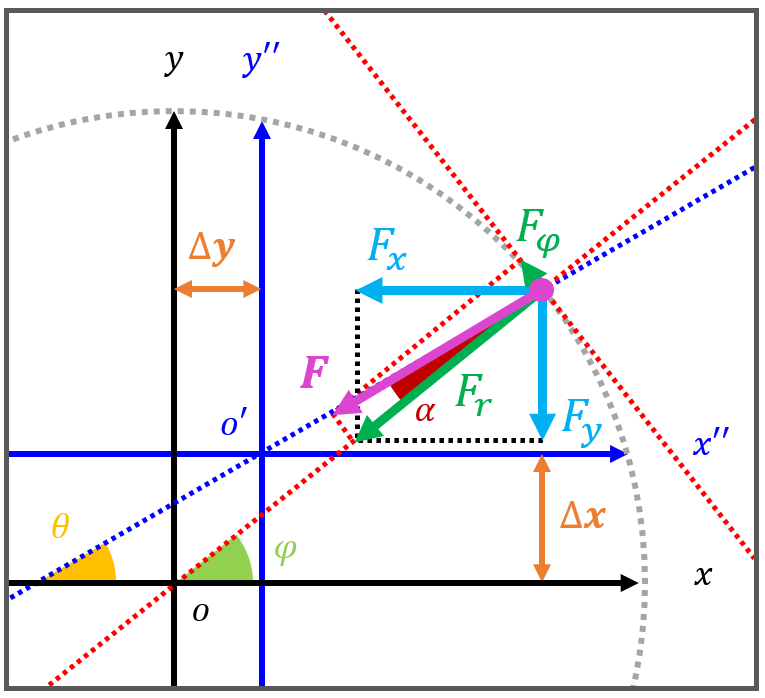
\includegraphics[width=75mm]{../images/34-1.png}
        \caption{}
    \end{center}
\end{figure}

\newpage

\subsubsection{角度$\alpha$の算出}
供試体の半径を$r$とするとき,作用点$F(x,y)$の座標は角度$\varphi$を用いて以下のように表すことができる.

\begin{align*}
    x & = r \cos \varphi \\
    y & = r \sin \varphi
\end{align*}
\vskip \baselineskip

また,座標系[2]において,作用点$F(x'',y'')$の座標はオフセット$\Delta x$,$\Delta y$を用いて
以下のように表される.

\begin{align*}
    x'' & = r \cos \varphi -\Delta x \\
    y'' & = r \sin \varphi -\Delta y
\end{align*}
\vskip \baselineskip

以上より,角度$\theta$を用いて角度$\varphi$を求めることができる.

\begin{align*}
    \tan \theta & = \frac{y''}{x''} = \frac{ r \sin \varphi - \Delta y}{ r \cos \varphi - \Delta x}      \\
    \notag                                                                                               \\
    \varphi     & = \theta - \sin^{-1}\left(\frac{\Delta x \sin \theta - \Delta y \cos \theta}{r}\right)
\end{align*}
\vskip \baselineskip

したがって,角度$\alpha$を以下のように求めることができる.

\begin{align*}
    \alpha = \theta - \varphi = \sin^{-1} \left( \frac{\Delta x \sin \theta - \Delta y \cos \theta}{r} \right)
\end{align*}
\vskip \baselineskip

\subsubsection{作用力$F$の分解}

供試体に加わる作用力$F$は供試体表面の接線方向の力$F_\varphi$,
またその法線方向の力$F_r$に分けて考えることができる.
ロードセルから与える作用力の角度$\theta$,算出した$\varphi$を用いると,それぞれ以下のように求められる.

\begin{align*}
    F_{\varphi} & = F \sin \alpha \\
    F_{r}       & = F \cos \alpha
\end{align*}
\vskip \baselineskip

供試体への作用力について抗力方向を$F_{x}$,揚力方向を$F_{y}$とすると
角度$\varphi$を用いて以下のように求められる.

\begin{align*}
    F_{x} & = - F_r \cos \varphi \\
    F_{y} & = - F_r \sin \varphi
\end{align*}
\vskip \baselineskip

また,接線方向成分$F_\varphi$について,供試体に対してトルク$T$として作用することとなる.

\begin{align*}
    T & = F_\varphi \cdot r = F \sin \alpha \cdot r
\end{align*}
\vskip \baselineskip

ここで,このトルク$T$について,
作用力測定装置に対する影響は十分に小さいと考えられることから無視できる.\\

\subsubsection{出力電圧勾配の座標系変換 (2)}

正規座標系に対して,オフセットを持つ座標系[2]を基準に
ロードセルから与えられる作用力$F$はすべて供試体に伝わることはなく,
接線方向の力$F_r$,その法線方向の力$F_\theta$に分解される.
すなわち,測定時にはロードセルから作用力$F$を与えた際の出力電圧,
ひずみセンサから作用力$F_r$を与えた際の出力電圧を得ているということになる.
したがって,ひずみセンサの出力電圧の傾きを一様に評価することは不可能であり,
実際の作用力$F_r$の角度$\alpha$を算出し補正を加える必要がある.

ここで,ひずみセンサの出力電圧$V_{x''2}$,$V_{y''2}$は
それぞれ$F_r / F$倍されていると考えられることから,
正規座標系における出力電圧勾配$v_{x}$,$v_{y}$と
座標系[2]における出力電圧勾配$v_{x''2}$,$v_{y''2}$は
角度$\alpha$を用いて以下のような関係が成立する.

\begin{align*}
    v_{x} & = \frac{F}{F_r} v_{x''2} = \frac{1}{\cos \alpha} v_{x''2} \\
    \notag                                                            \\
    v_{y} & = \frac{F}{F_r} v_{y''2} = \frac{1}{\cos \alpha} v_{y''2}
\end{align*}

\newpage

\subsection{複合状態における補正理論}
\vskip \baselineskip

\subsubsection{補正理論の適用順序}

作成した補正理論について,座標系の回転角$\theta_x$,$\theta_y$の特定の際に
離散フーリエ変換を適用することから,座標系のオフセットにおける補正理論を先に適用する必要がある.
ここで,オフセットを考慮した場合,データ間隔が不等間隔となるため
回転角を特定するための離散フーリエ変換が適用できない.
したがって,ラグランジュ補間を用いて二次近似を行い,等間隔のデータを補完することとした.\\

\subsubsection{ラグランジュ補間}

ラグランジュ補間とは,一般的に以下のように表される.

\begin{align*}
    P\left(x\right)    & = \sum^{n+1}_{i=1} y_i \frac{f_i\left(x\right)}{f_i \left(x_i\right)} \\
    f_i \left(x\right) & = \prod_{k \neq i} \left(x - x_k\right)
\end{align*}
\vskip \baselineskip

ここで,2次補間を行う場合,使用する3点を適切に選択する必要があるが
アルゴリズムを用いて処理を行いたい.
そこで,以下のような手順でラグランジュ補間を行った.\\

\subsubsection{使用するデータの選択}

性能評価実験では,15度ずつ測定しているため,計24点のデータを得ることができる.
座標系のオフセットにおける補正理論を用いた補正処理では,正規座標系における作用力とその角度が算出される.
しかし,離散フーリエ変換を適用するとき,等間隔のデータが必要となるため15度ごとの補間値を算出しなければならない.
ここで,必要な補間値の角度を$\theta$とするとき,
実際の作用力の角度$\varphi$との差
$\delta \theta$を絶対値で評価することで,その値$|\delta \theta|$が
最も小さくなる角度$\varphi$とその前後のデータを使用することで,$\theta$に最も近い3点を選択することができる.

\begin{align*}
    \delta \theta = |\theta - \varphi|
\end{align*}

\subsubsection{テストデータへの適用 (3)}
上述の補正理論より座標系の回転・オフセットを考慮したテストデータを作成する.
任意の回転角$\theta_{1\;\mathrm{test}}$,$\theta_{2\; \mathrm{test}}$,
任意のオフセット$\Delta x_\mathrm{test}$,$\Delta y_\mathrm{test}$を与え,
複合状態における出力電圧勾配について,$x''$軸方向を$v_{x''\;\mathrm{test}}$,
$y''$軸方向を$v_{y''\;\mathrm{test}}$とするとき,以下のように表される.

\begin{align*}
    \theta                  & = \frac{\pi}{180} \; i \;\left(i = 0, 1, 2, 3, \cdots\right)                                                       \\
    \alpha                  & = \sin^{-1} \left( \frac{\Delta x_\mathrm{test} \sin \theta - \Delta y_\mathrm{test} \cos \theta}{r} \right)       \\
    \varphi                 & = \theta - \sin^{-1}\left(\frac{\Delta x_\mathrm{test} \sin \theta - \Delta y_\mathrm{test} \cos \theta}{r}\right) \\
    \notag                                                                                                                                       \\
    v_{x'' \;\mathrm{test}} & = - \cos \alpha \cos \left(\varphi - \theta_{1\; \mathrm{test}} \right)                                            \\
    v_{y'' \;\mathrm{test}} & = - \cos \alpha \sin \left(\varphi - \theta_{2\; \mathrm{test}}\right)
\end{align*}

また,今回を以下のTable 2のようなパラメータを用いた.

\begin{table}[htbp]
    \begin{center}
        \caption{Test data conditions (3)}
        \begin{tabular}{|p{20mm}|p{20mm}|p{20mm}|p{20mm}|}
            \hline
            \multicolumn{1}{|c|}{$\theta_{1\;\mathrm{test}}$ [deg]} & \multicolumn{1}{|c|}{$\theta_{2\;\mathrm{test}}$ [deg]} & \multicolumn{1}{|c|}{$\Delta x_\mathrm{test}$ [mm]} & \multicolumn{1}{|c|}{$\Delta y_\mathrm{test}$ [mm]} \\ \hline
            \multicolumn{1}{|c|}{10.0}                              & \multicolumn{1}{|c|}{-5.0}                              & \multicolumn{1}{|c|}{5.00}                          & \multicolumn{1}{|c|}{-2.50}                         \\ \hline
        \end{tabular}
    \end{center}
\end{table}

はじめに,作成したテストデータを以下に示す.

\begin{figure}[htbp]
    \footnotesize
    \begin{center}
        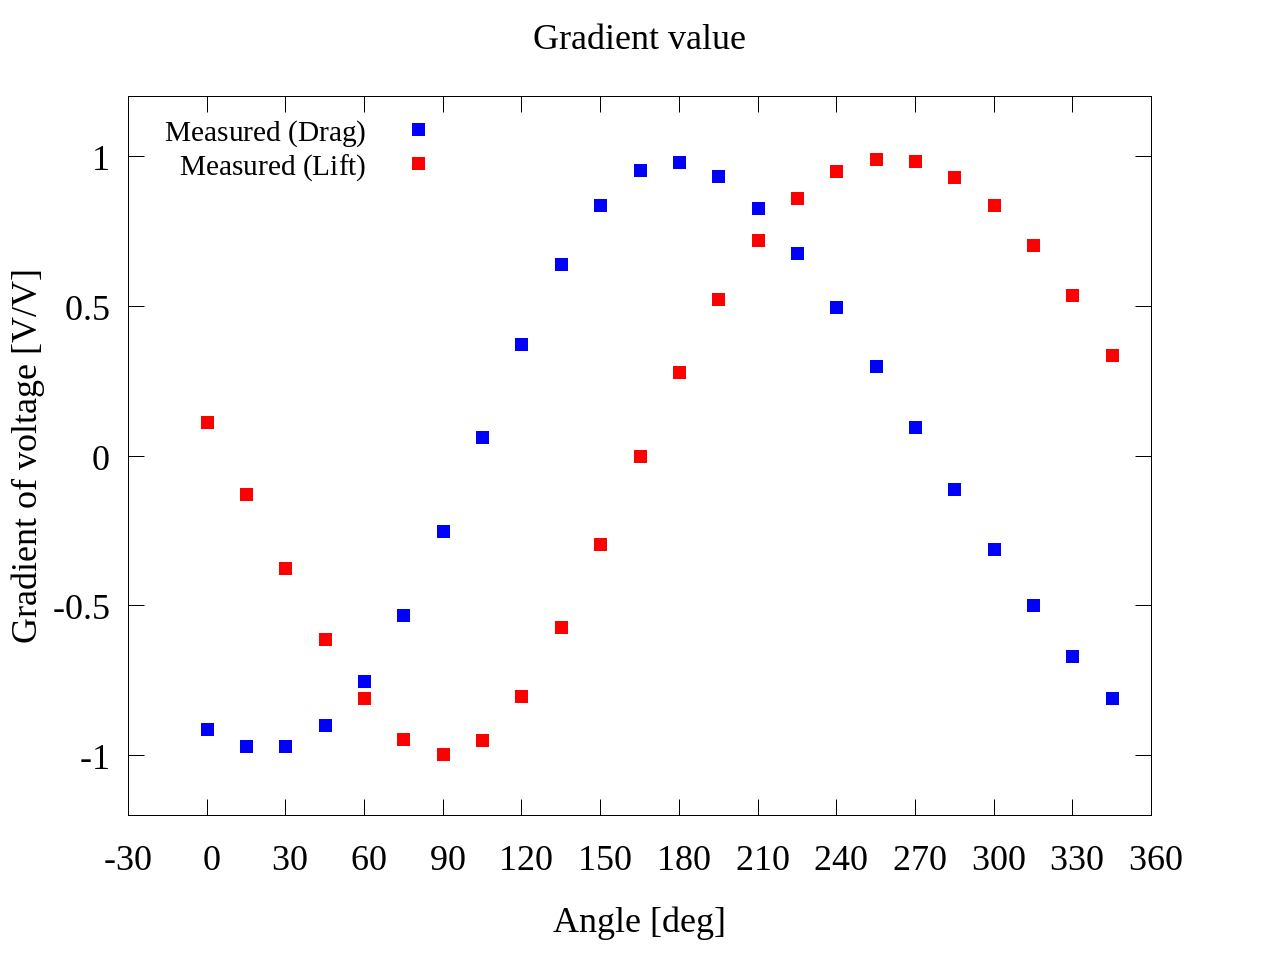
\includegraphics[width=82mm]{../../../02_workspace/result/simulation_tx=10.0_ty=-5.0_dx=5.00_dy=-2.50/plot/05/05_summary-wave.png}
        \caption{Simulated data}
    \end{center}
\end{figure}

ここで,座標系のオフセットにおける補正理論を適用した結果を以下のFig.15,Fig.16に示す.

\begin{figure}[htbp]
    \begin{center}
        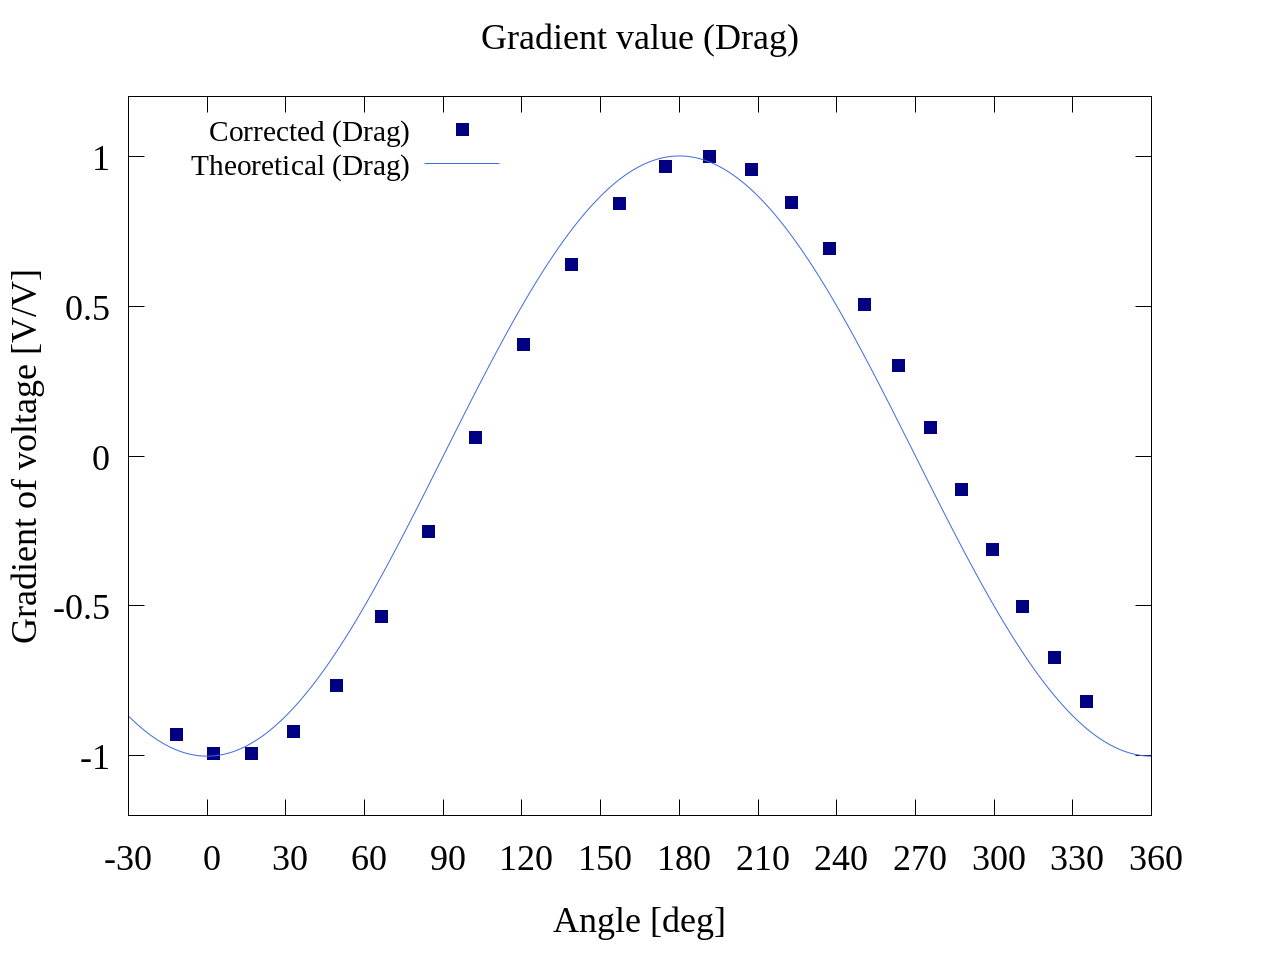
\includegraphics[width=82mm]{../../../02_workspace/result/simulation_tx=10.0_ty=-5.0_dx=5.00_dy=-2.50/plot/21/21-2_corrected_offset_drag.png}
        \caption{Offset corrected value (Drag)}
        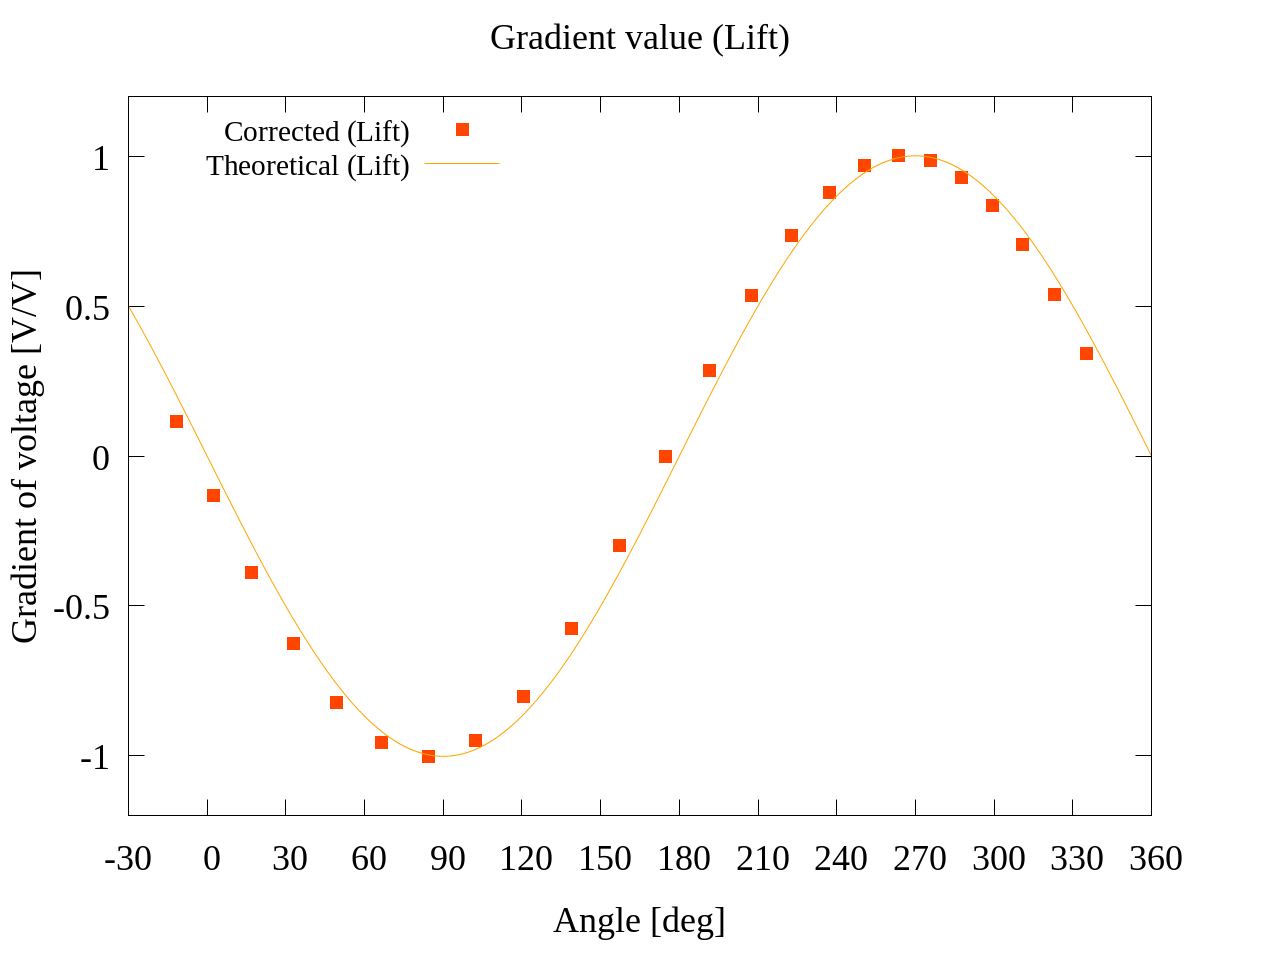
\includegraphics[width=82mm]{../../../02_workspace/result/simulation_tx=10.0_ty=-5.0_dx=5.00_dy=-2.50/plot/21/21-2_corrected_offset_lift.png}
        \caption{Offset corrected value (lift)}
    \end{center}
\end{figure}

\newpage

理論曲線と比較して,波形の再現はされているが,位相差があるようにみえる.
また,プロットされたデータ間隔は異なることもわかる.
このとき,ラグランジュ補間を用いて,等間隔のデータを得るための処理を行う.
なお,データの採用点については上述の処理によって行うこととする.
ラグランジュ補間を行った結果を以下のFig.17,Fig.18に示す.

\begin{figure} [htbp]
    \begin{center}
        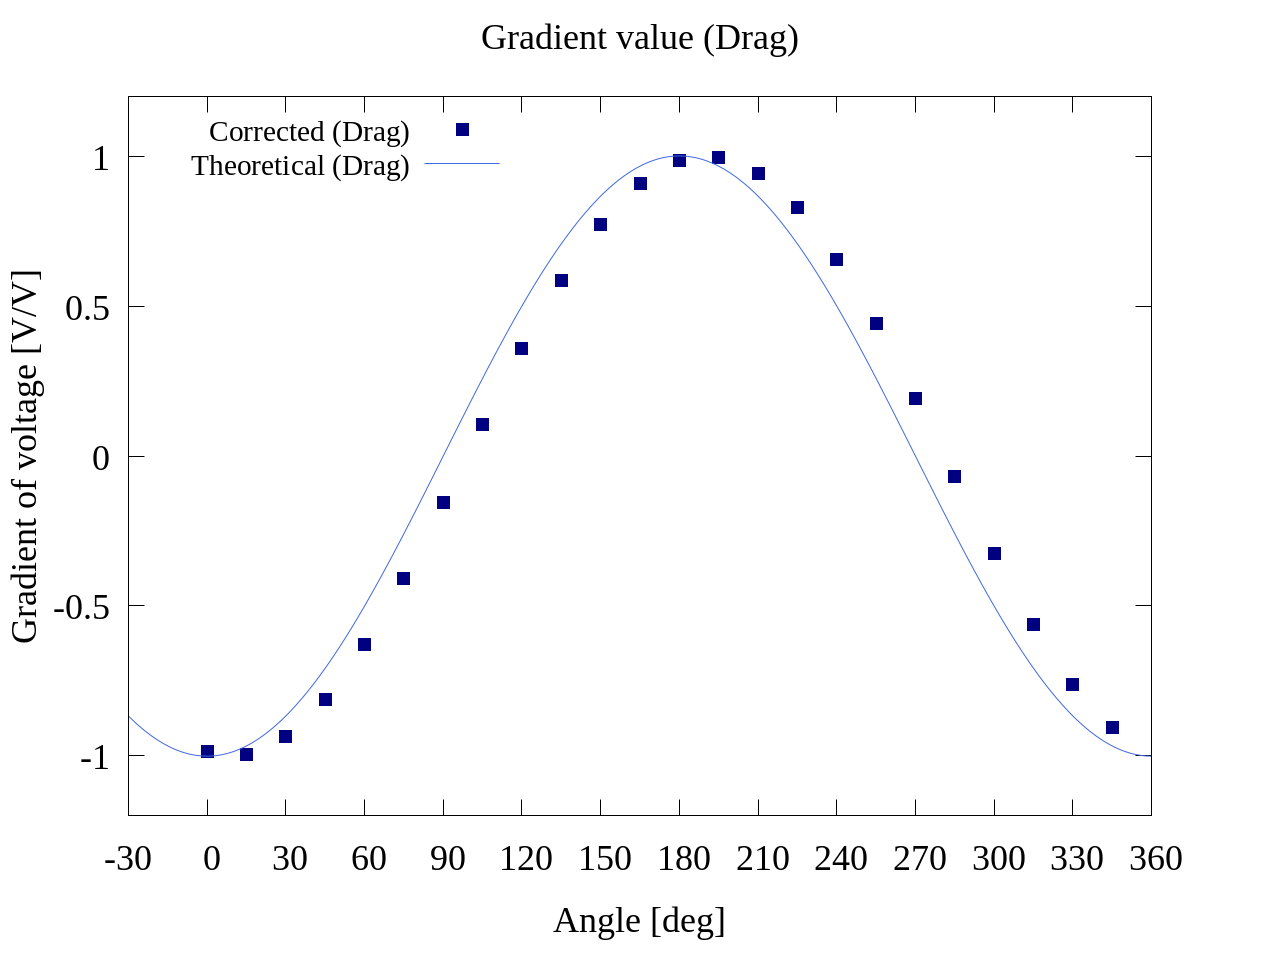
\includegraphics[width=82mm]{../../../02_workspace/result/simulation_tx=10.0_ty=-5.0_dx=5.00_dy=-2.50/plot/21/21-3_interpolated_drag.png}
        \caption{Offset corrected value (Drag)}
        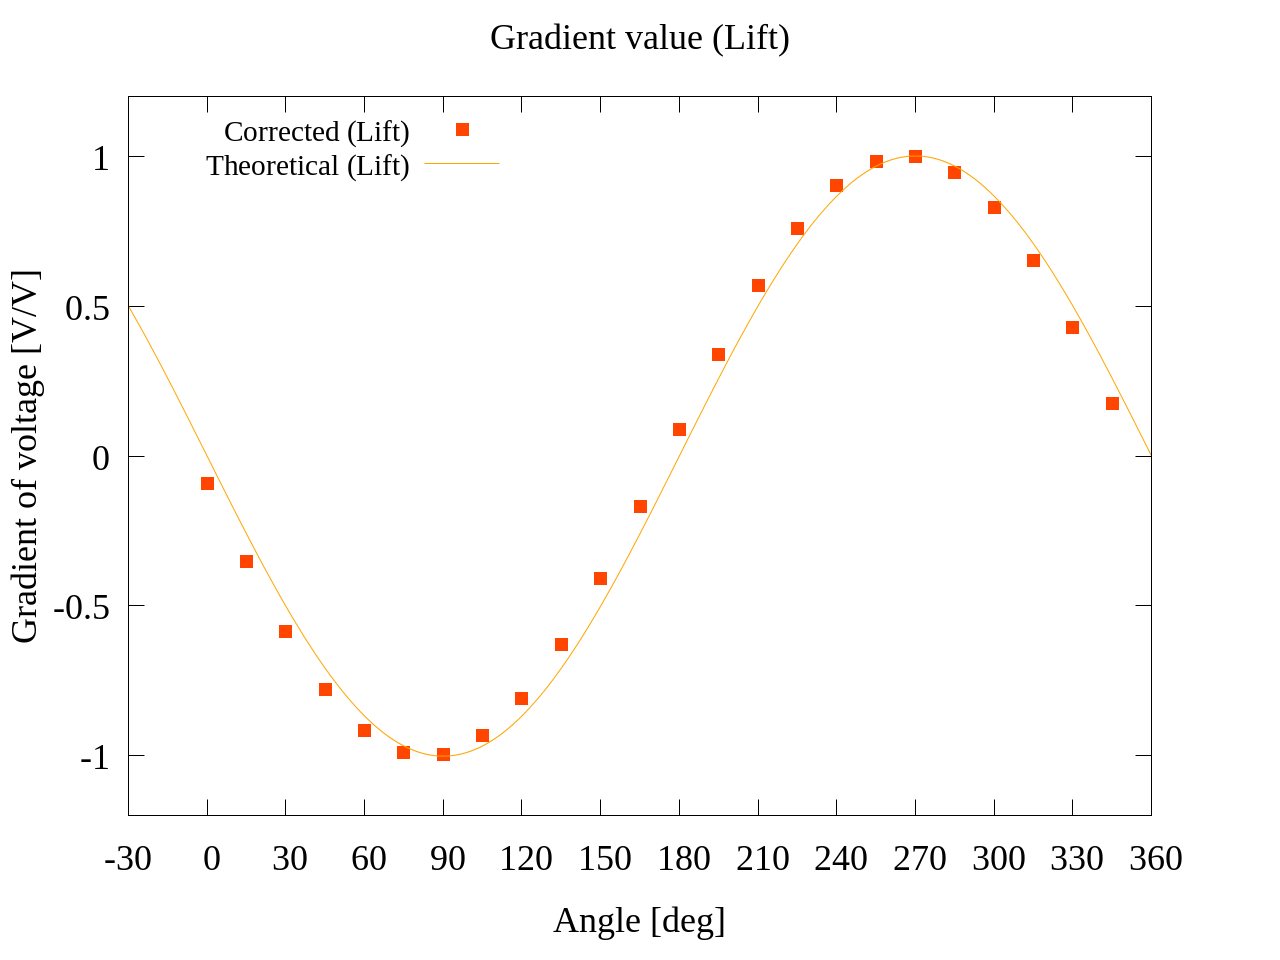
\includegraphics[width=82mm]{../../../02_workspace/result/simulation_tx=10.0_ty=-5.0_dx=5.00_dy=-2.50/plot/21/21-3_interpolated_lift.png}
        \caption{Offset corrected value (lift)}
    \end{center}
\end{figure}

\newpage

上記のFig.17,Fig.18と比較すると等間隔のデータを得られていることがわかる.
次に,フーリエ変換を適用する.
このときの結果を以下のFig.19,Fig.20 に示す.
また,波数1の成分についての算出値を以下のTable 3に示す.

\begin{table}[htbp]
    \begin{center}
        \caption{DFT result value}
        \begin{tabular}{|p{30mm}|p{20mm}|p{20mm}|}
            \hline
            \multicolumn{1}{|c|}{}     & \multicolumn{1}{|c|}{$Re$}    & \multicolumn{1}{|c|}{$Im$}   \\ \hline
            \multicolumn{1}{|c|}{Drag} & \multicolumn{1}{|c|}{-11.835} & \multicolumn{1}{|c|}{2.083}  \\ \hline
            \multicolumn{1}{|c|}{Lift} & \multicolumn{1}{|c|}{-1.081}  & \multicolumn{1}{|c|}{11.978} \\ \hline
        \end{tabular}
    \end{center}
\end{table}

\newpage
\begin{figure}[htbp]
    \begin{center}
        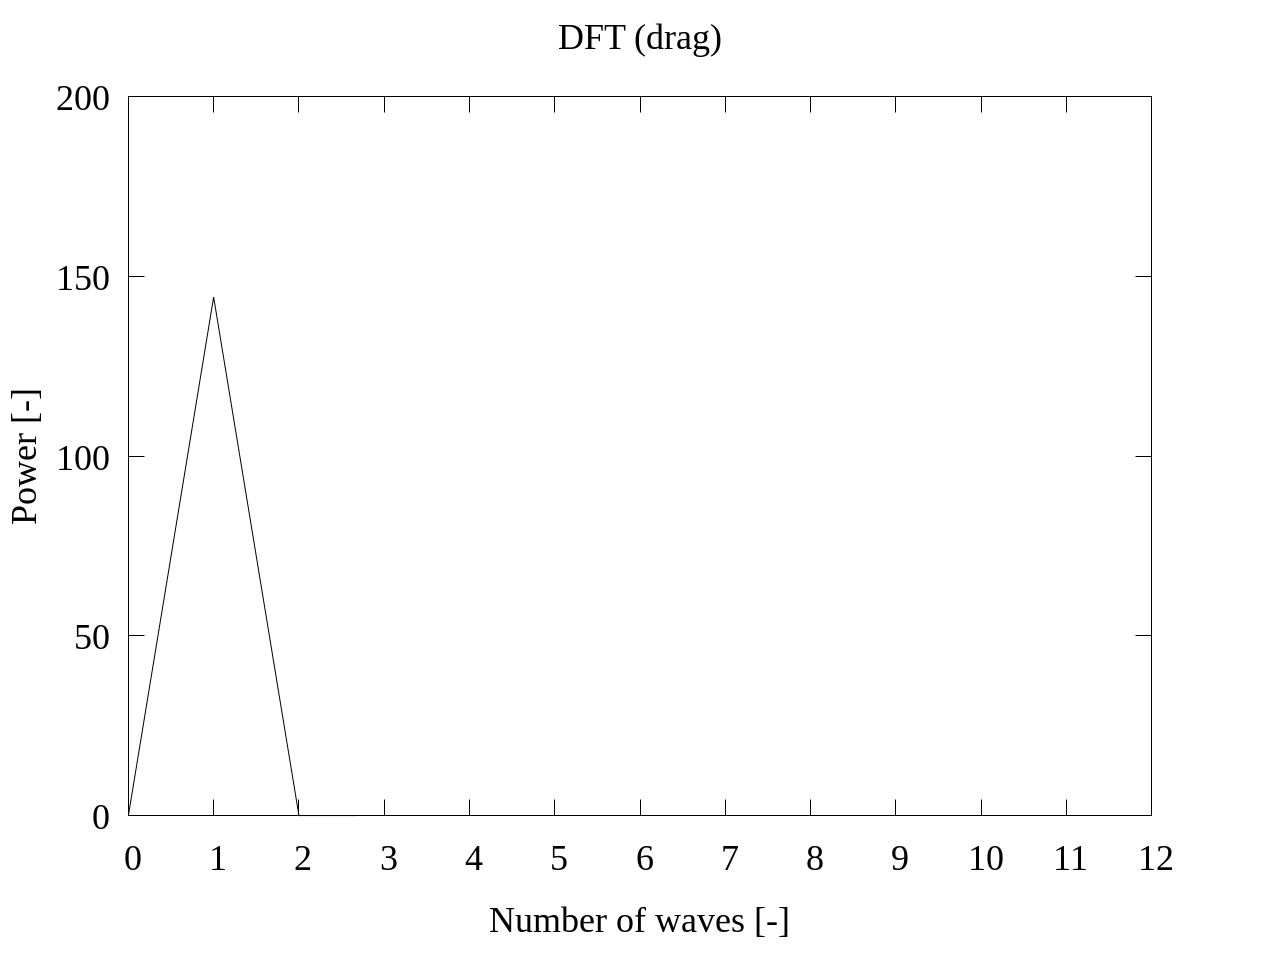
\includegraphics[width=82mm]{../../../02_workspace/result/simulation_tx=10.0_ty=-5.0_dx=5.00_dy=-2.50/plot/07/07-3_dft-drag.png}
        \caption{DFT result (Drag)}
        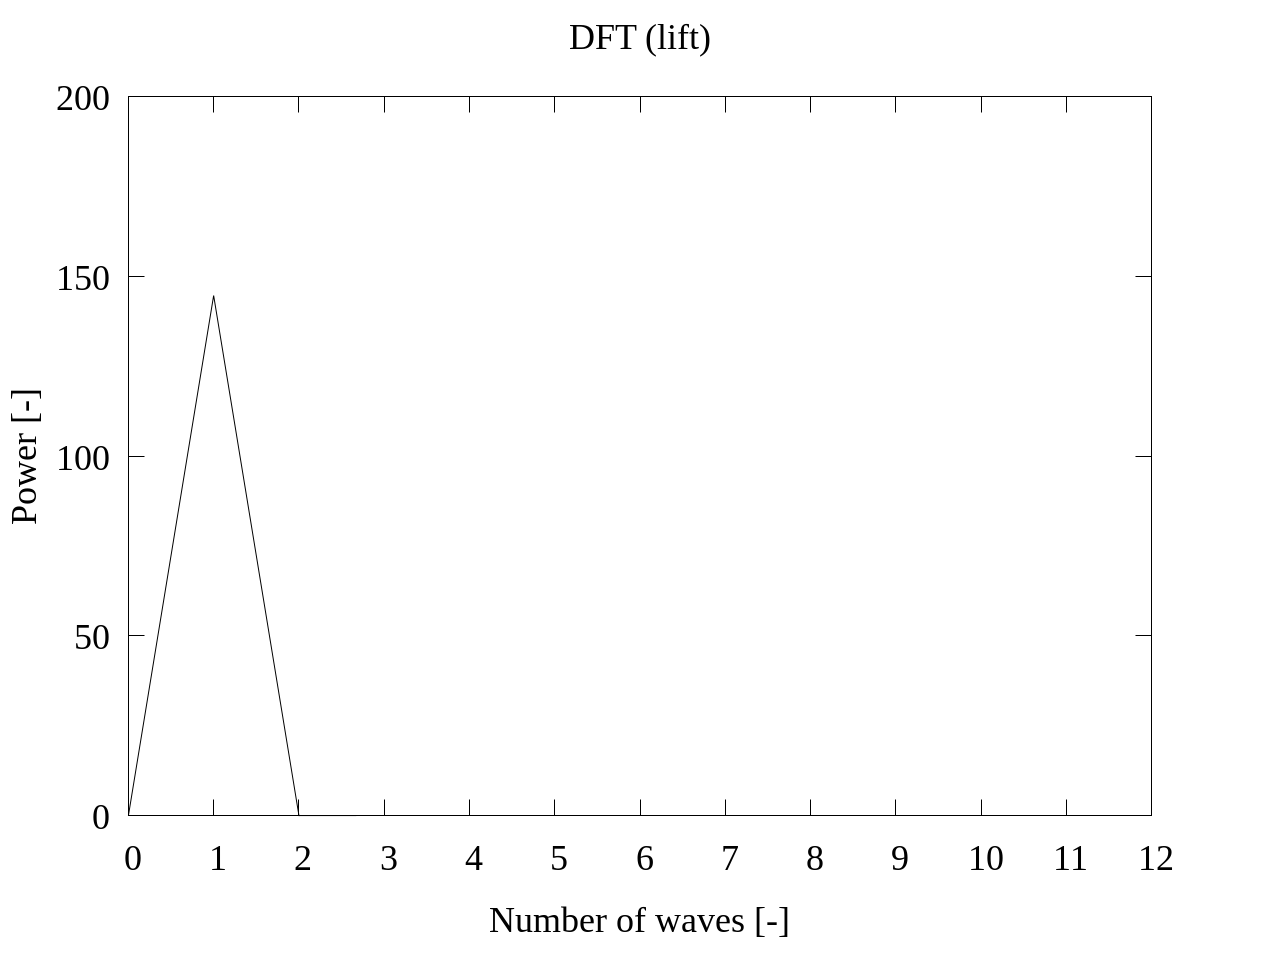
\includegraphics[width=82mm]{../../../02_workspace/result/simulation_tx=10.0_ty=-5.0_dx=5.00_dy=-2.50/plot/07/07-4_dft-lift.png}
        \caption{DFT result (lift)}
    \end{center}
\end{figure}

Fig.19,Fig.20 より,波数1についてピークがあることがわかり,
座標軸の回転における補正理論の適用結果と同様にデータの特徴を正しく捉えられているといえる.
ここで,Table 4 について,回転角$\theta_x$,$\theta_y$をそれぞれ算出する.

\begin{table}[htbp]
    \begin{center}
        \caption{Specified rotation angle}
        \begin{tabular}{|p{30mm}|p{20mm}|p{20mm}|}
            \hline
            \multicolumn{1}{|c|}{$\theta_x$ [deg]} & \multicolumn{1}{|c|}{$\theta_y$ [deg]} \\ \hline
            \multicolumn{1}{|c|}{10.018}           & \multicolumn{1}{|c|}{-5.158}           \\ \hline
        \end{tabular}
    \end{center}
\end{table}

結果より,算出された回転角$\theta_{1\;\mathrm{test}}$,$\theta_{2\;\mathrm{test}}$は
Table 2で設定したパラメータと比較すると,異なっていることがわかる.
これは,ラグランジュ補間公式を用いた2次近似による誤差が生じているためと考えられる.

算出した回転角$\theta_{1\;\mathrm{test}}$,$\theta_{2\;\mathrm{test}}$を用いて
座標系の回転における補正理論を適用した結果を以下のFig.21,Fig.22,に示す.

\newpage

\begin{figure}[htbp]
    \footnotesize
    \begin{center}
        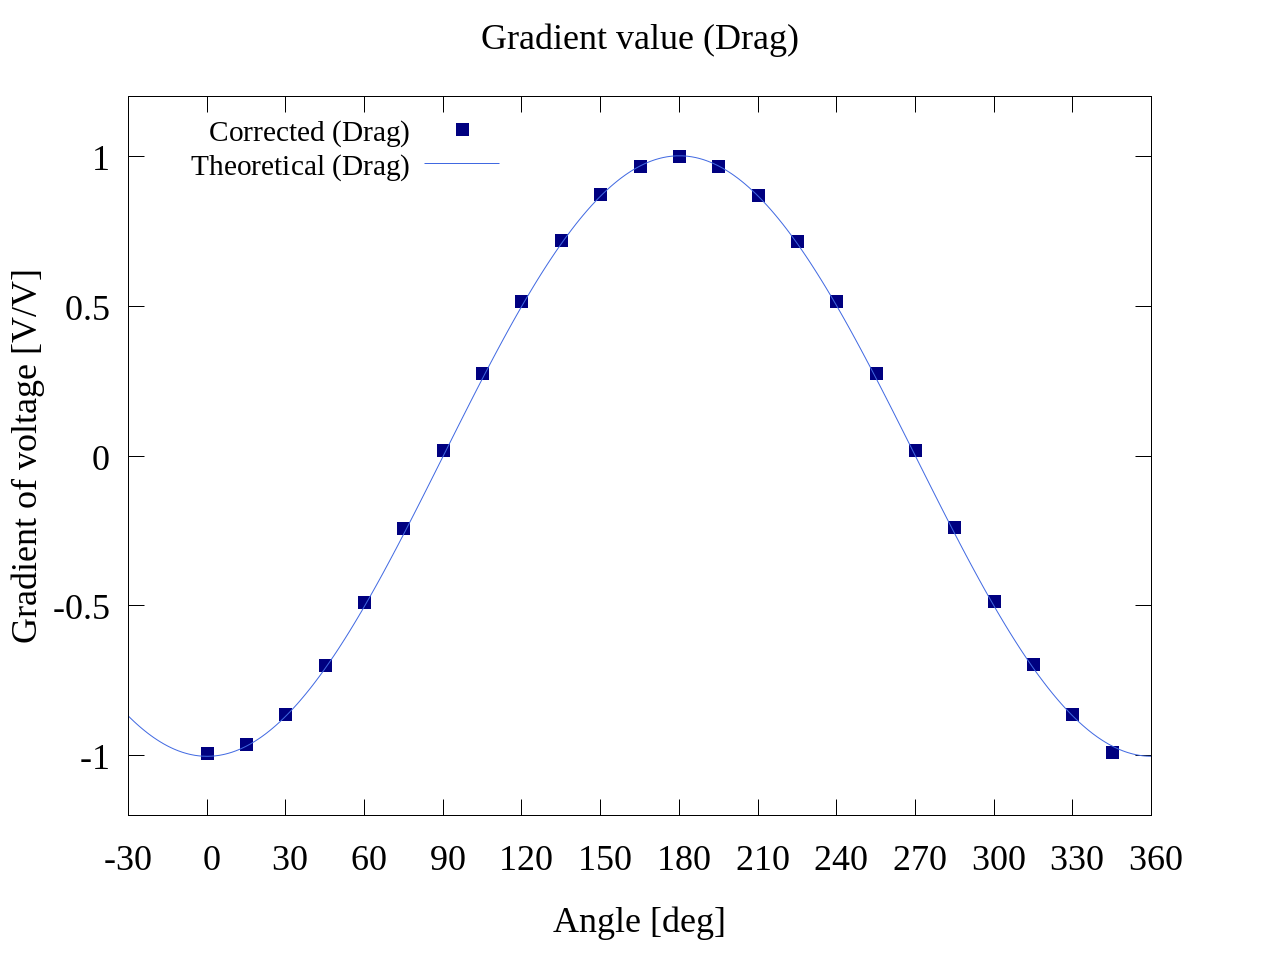
\includegraphics[width=82mm]{../../../02_workspace/result/simulation_tx=10.0_ty=-5.0_dx=5.00_dy=-2.50/plot/21/21-4_corrected_angle_drag.png}
        \caption{interpolated data (Drag)}
        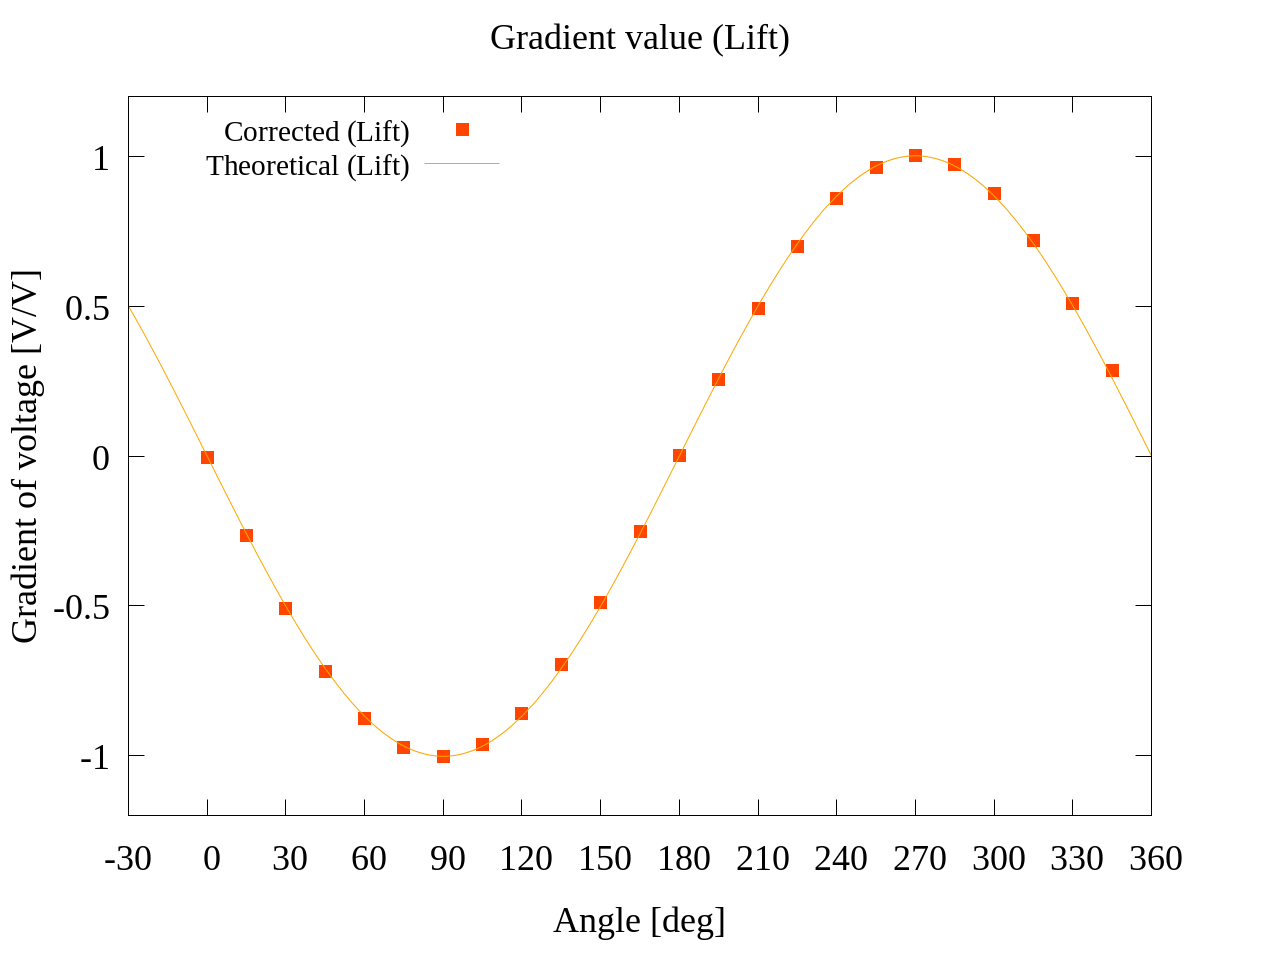
\includegraphics[width=82mm]{../../../02_workspace/result/simulation_tx=10.0_ty=-5.0_dx=5.00_dy=-2.50/plot/21/21-4_corrected_angle_lift.png}
        \caption{interpolated data (Lift)}
    \end{center}
\end{figure}

また,以下の式を用いて算出した正味出力電圧勾配$v_{\mathrm{net}}$を以下のFig.23に示す.

\begin{align*}
    v_{\mathrm{net}} & = \sqrt{v_d^2 + v_l^2}
\end{align*}

\begin{figure}[htbp]
    \footnotesize
    \begin{center}
        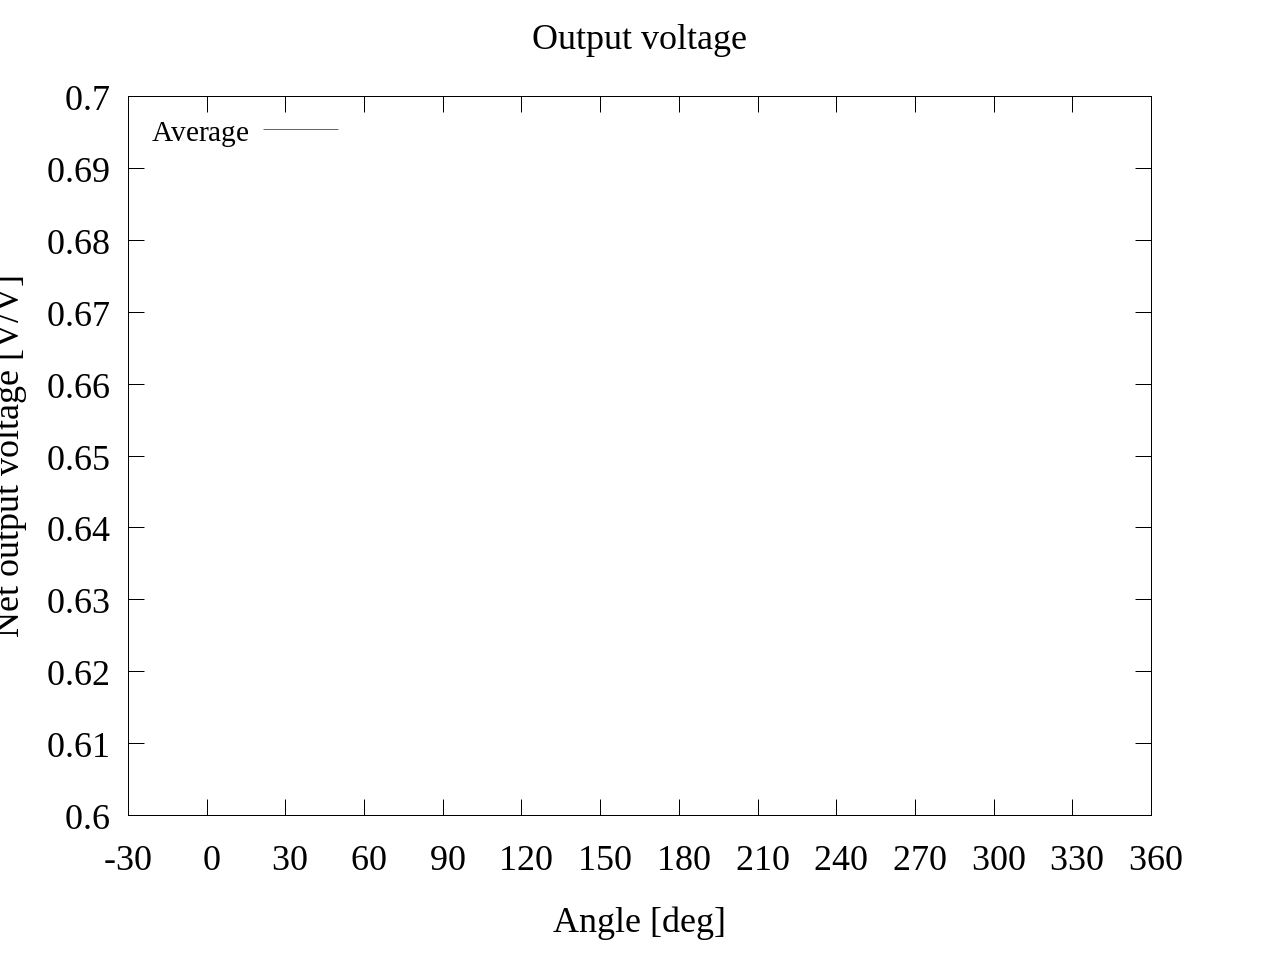
\includegraphics[width=82mm]{../../../02_workspace/result/simulation_tx=10.0_ty=-5.0_dx=5.00_dy=-2.50/plot/09/09_summary-outputvoltage-net.png}
        \caption{Net output voltage (test data)}
    \end{center}
\end{figure}

\newpage

ここで,正味出力電圧勾配とは,テストデータにおける市ぷくの大きさを表しており,
その値は1としてテストデータは作成されている.
Fig.23 をみるとラグランジュ補間による影響から値が変動しているものの
おおよその値はどの角度においても1を示していることがわかる.
したがって,上述のホセ理論は正常に動作しているといえる.

\section{補正理論の適用結果}

ここで,上述の補正理論を実験結果への適用結果を以下のFig.24,Fig.25に示す.

\begin{figure}[htbp]
    \begin{center}
        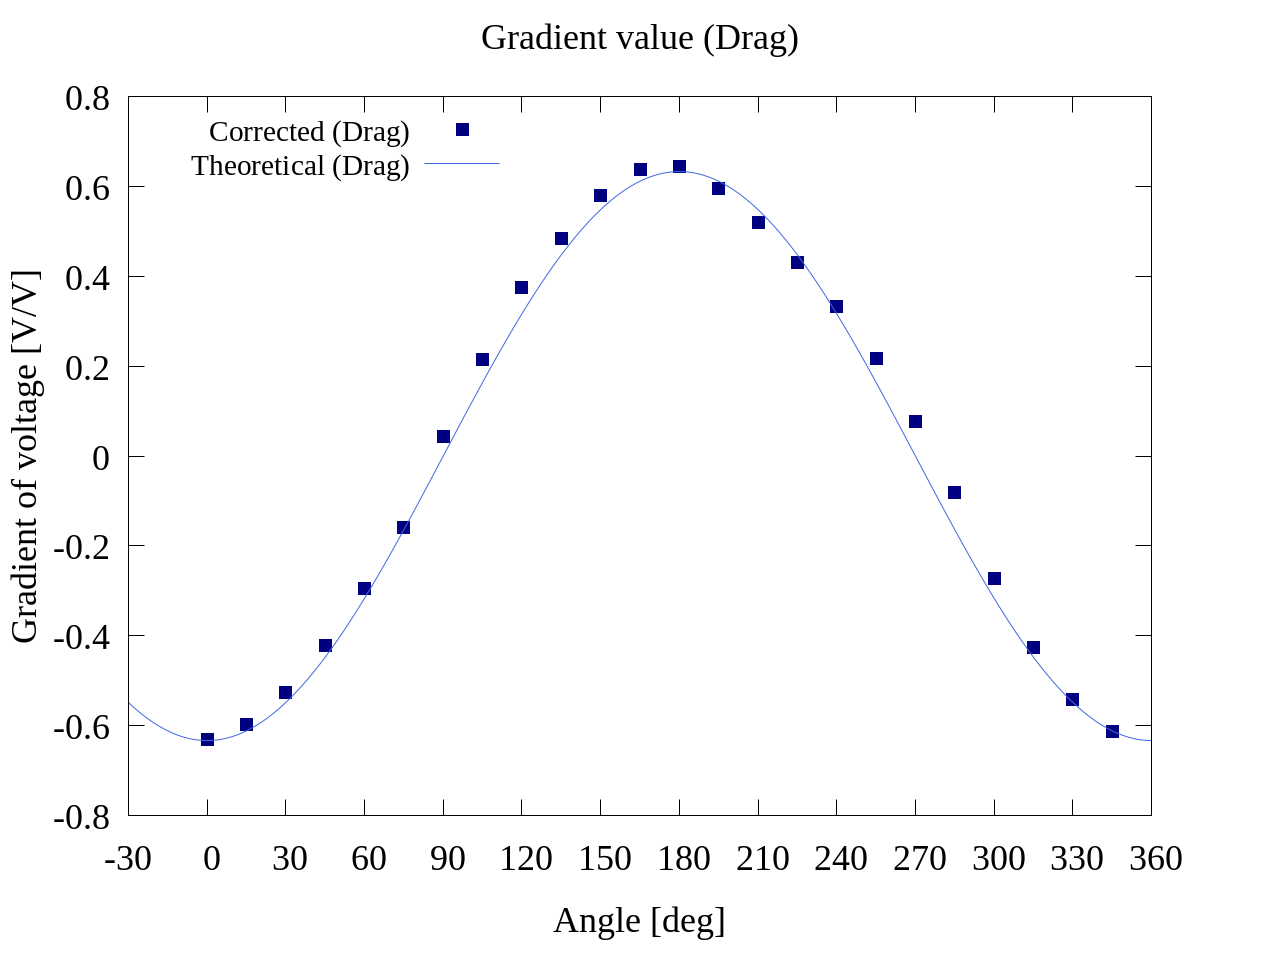
\includegraphics[width=82mm]{../../../02_workspace/result/2-ex/plot/21/21-4_corrected_angle_drag.png}
        \caption{Corrected result (Drag)}
        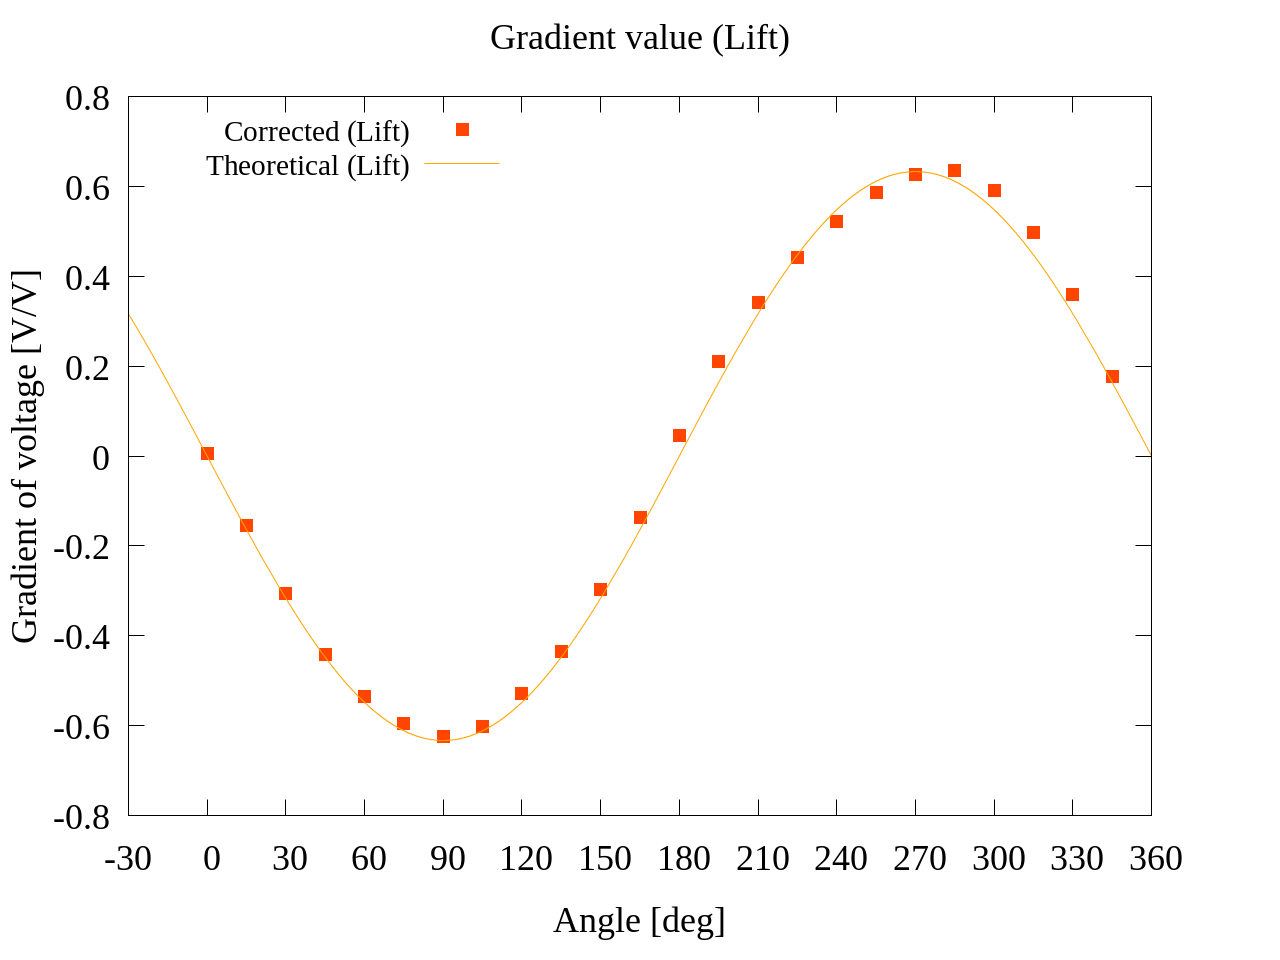
\includegraphics[width=82mm]{../../../02_workspace/result/2-ex/plot/21/21-4_corrected_angle_lift.png}
        \caption{Corrected result (lift)}
    \end{center}
\end{figure}

Fig.24,Fig.25をみると理論曲線に対しておおよその波形は一致しているようにみえる.
しかし,180度以降理論曲線から大きく外れているデータもみられる.
したがって,今後この補正値と理論曲線についての評価方法を検討する必要がある.

\newpage

また,算出した正味出力電圧勾配を以下のFig.26に示す.

\begin{figure}[htbp]
    \begin{center}
        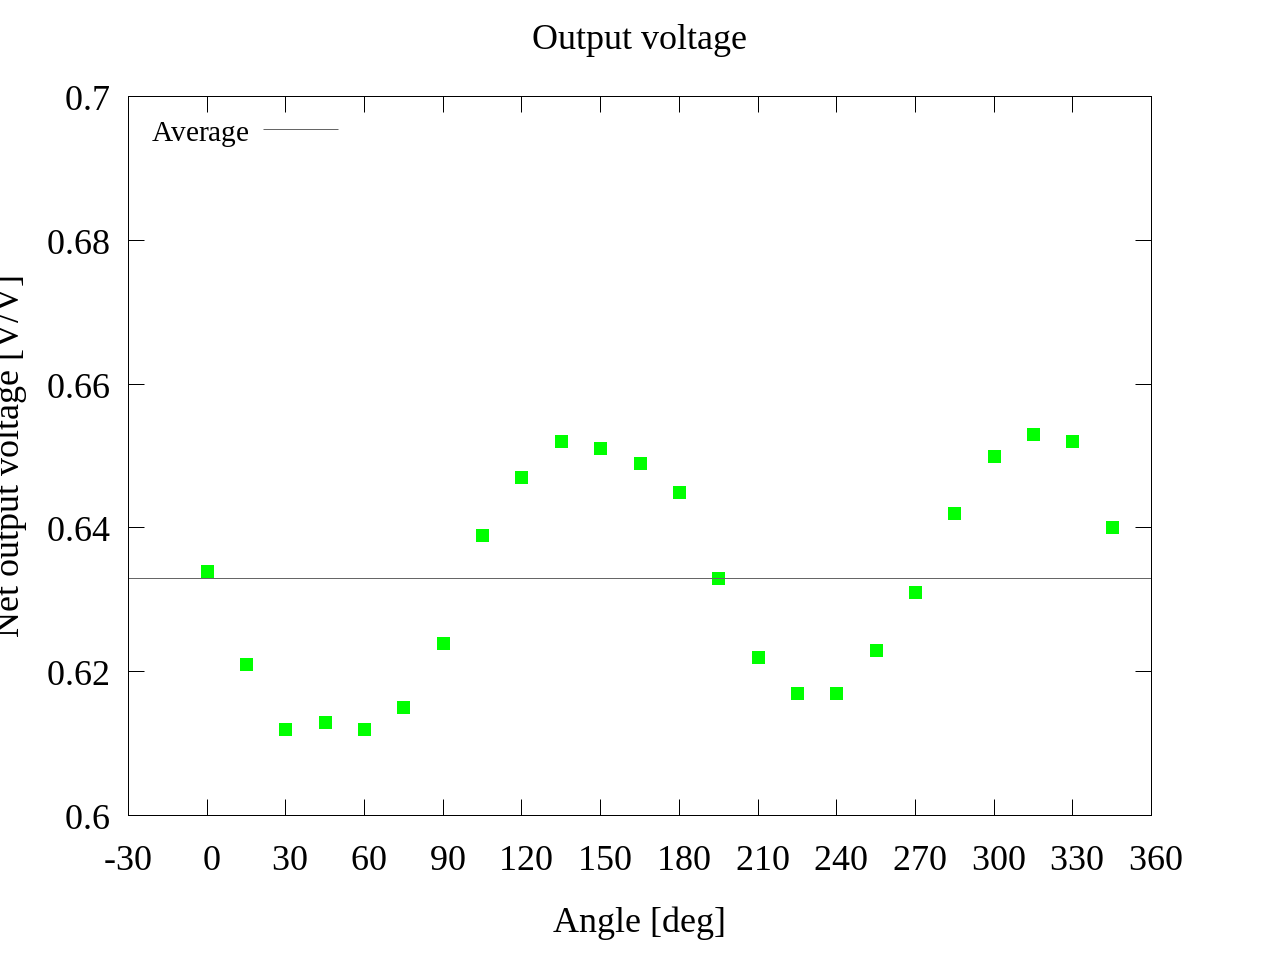
\includegraphics[width=82mm]{../../../02_workspace/result/2-ex/plot/09/09_summary-outputvoltage-net.png}
        \caption{Net gradient of voltage}
    \end{center}
\end{figure}

ここで,Fig.26をみると周期的な振動を確認できる.
本来,正味出力電圧は一定であると考えることができるため,
他の要因によって影響を受けていることが考えられる.
今後はこの波形が生じる要因を検討し,補正理論へ組み込むことを考えている.


\section{今月のまとめと今後の予定}
\begin{itemize}
    \item [$\blacksquare$] 今月のまとめ
          \begin{itemize}
              \item [$\bullet$] 製作した実験装置を用いて性能評価実験を行った
              \item [$\bullet$] 自動化することで,人為的操作による非再現性を取り除き,
                    実験回数を大幅に向上することができた
              \item [$\bullet$] 実験結果の補正理論を作成しデータ処理を行った
              \item [$\bullet$] テストデータへの補正理論適用結果から
                    おおよそ問題がないことが確認できた
              \item [$\bullet$] 2ゲージ法による影響を考慮する必要があることがわかった.
          \end{itemize}
          \vskip\baselineskip
    \item [$\blacksquare$] 2月の予定
          \begin{itemize}
              \item [$\bullet$] 卒業論文の執筆
              \item [$\bullet$] 実験の実施 (1月末まで)
              \item [$\bullet$] 補正適用結果の評価方法の検討
              \item [$\bullet$] 新たな補正方法の検討
          \end{itemize}
\end{itemize}
\end{document}